%This file is part of diplom-kovalev
%Copyright (C) 2012 Maxim Kovalev.
%Permission is granted to copy, distribute and/or modify this document
%under the terms of the GNU Free Documentation License, Version 1.3
%or any later version published by the Free Software Foundation;
%with no Invariant Sections, no Front-Cover Texts, and no Back-Cover Texts.
%A copy of the license is included in the section entitled "GNU
%Free Documentation License".

\documentclass{beamer}
\usepackage{beamerthemesplit}
\usepackage[T2A,T1]{fontenc}
\usepackage[utf8]{inputenc}
\usepackage[english,russian]{babel}
\usepackage{graphicx}
\graphicspath{{images/}}
\usepackage{caption}
\usepackage{subcaption}
\usepackage{cmap}
\usepackage{multirow}
%\setbeamertemplate{footline}[frame number]
\usepackage{listings}
\lstset{language=Python}

\makeatletter
\setbeamertemplate{footline}
{
  \leavevmode%
  \hbox{\large%
  \begin{beamercolorbox}[wd=.3\paperwidth,ht=2.25ex,dp=1ex,center]{author in head/foot}%
    \usebeamerfont{author in head/foot}\insertshortauthor
  \end{beamercolorbox}%
  \begin{beamercolorbox}[wd=.59\paperwidth,ht=2.25ex,dp=1ex,center]{title in head/foot}%
    \usebeamerfont{title in head/foot}\insertshorttitle
  \end{beamercolorbox}%
  \begin{beamercolorbox}[wd=.11\paperwidth,ht=2.25ex,dp=1ex,right]{date in head/foot}%
	\insertframenumber/\inserttotalframenumber\hspace*{2ex}
  \end{beamercolorbox}}%
  \vskip0pt%
}
\makeatother

\setbeamertemplate{frametitle}
{\vskip-2pt
  \leavevmode
  \hbox{%
  \begin{beamercolorbox}[wd=\paperwidth,ht=3ex,dp=1ex]{frametitle}%
    \raggedright\hspace*{1em}{\bf{}\huge\insertframetitle}
  \end{beamercolorbox}
  }%
}



\title[GSM-позиционирование транспорта]{Разработка системы позиционирования общественного транспорта по сигналам сотовых сетей}
\subtitle{\texttt{http://svn.auditory.ru/repos/tatmon/}}
\author[Максим Ковалев]{Автор: Максим Максимович Ковалев \\ \texttt{maxim.kovalev@2007.auditory.ru} \\\vspace{1em} Руководитель: Дмитрий Олегович Столяров \\ \texttt{dmitry.stolyarov@gmail.com}}
\institute[МИЭМ]{Московский Государственный Институт Электроники и Математики (Технический Университет)\\ Кафедра ИКТ}
\date{6 июня 2012 г.}

\begin{document}

\frame{\titlepage}

\frame{
	\frametitle{Цели работы}
	\begin{columns}[T]
		\column{0.5\textwidth}
		\begin{itemize}
			\item
				{\bf Высшая} --- удобство перемещения по городу!
			\item
				Создать новую хорошую систему позиционирования;
			\item
				Отказаться от спутникового позиционирования;
			\item
				Повысить точность триангуляции по вышкам GSM.
				\begin{itemize}
					\item
						Проверить изобретённый метод.
				\end{itemize}
		\end{itemize}
		\column{0.5\textwidth}
		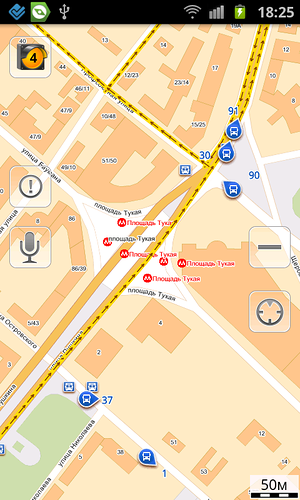
\includegraphics[height=0.7\textheight]{yakazan.png}

		Автобусы Казани в реальном времени на телефоне.
	\end{columns}
}

\frame{
	\frametitle{Архитектура системы}
	\center{
		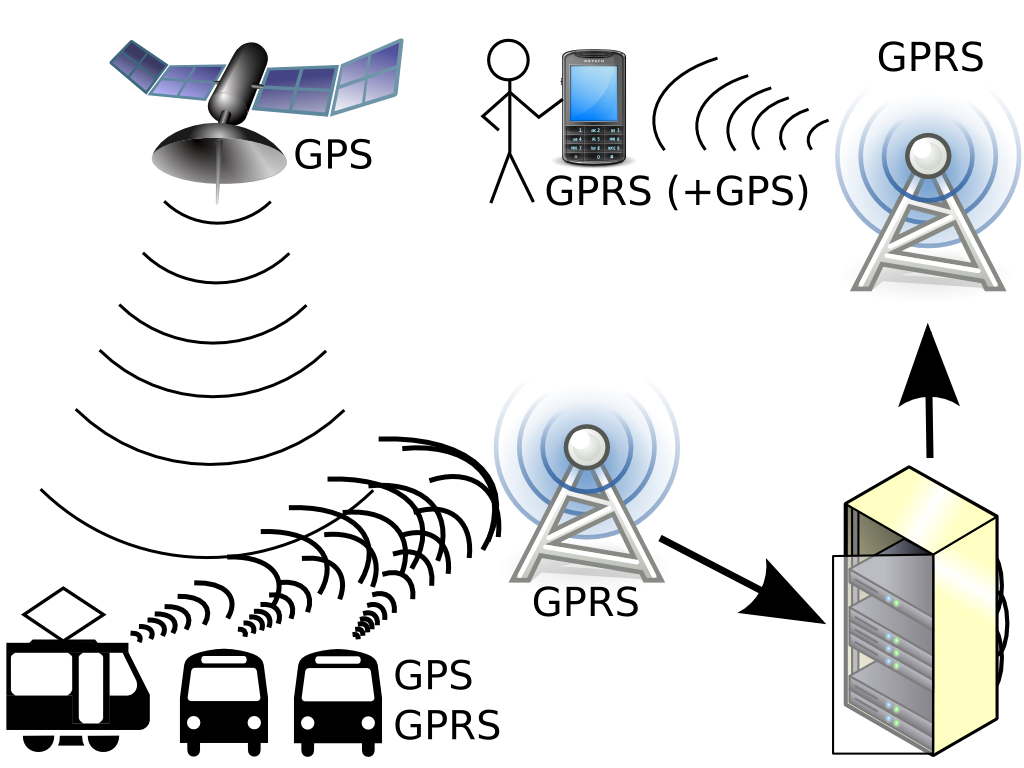
\includegraphics[width=0.9\textwidth]{general-arch-pict.png}
	}
}

\frame{
	\frametitle{Методы позиционирования}
	\begin{columns}[c]
		\column{0.5\textwidth}
		Спутниковая
		\begin{itemize}
			\item
				Спутники
			\item
				Время прохождения сигнала
			\item
				Строго и однозначно
			\item
				1 -- 50 метров погрешности
		\end{itemize}
		\column{0.5\textwidth}
		Сотовые сети
		\begin{itemize}
			\item
				Базовые станции
			\item
				Уровень сигнала
			\item
				Машинное обучение
			\item
				10 -- 500 метров погрешности
		\end{itemize}
	\end{columns}
}
\frame{
	\frametitle{Гипотеза}
	Триангуляция в сетях GSM недостаточно точна из-за чрезмерной экстраполяции.
	\begin{columns}[T]
		\column{0.5\textwidth}
		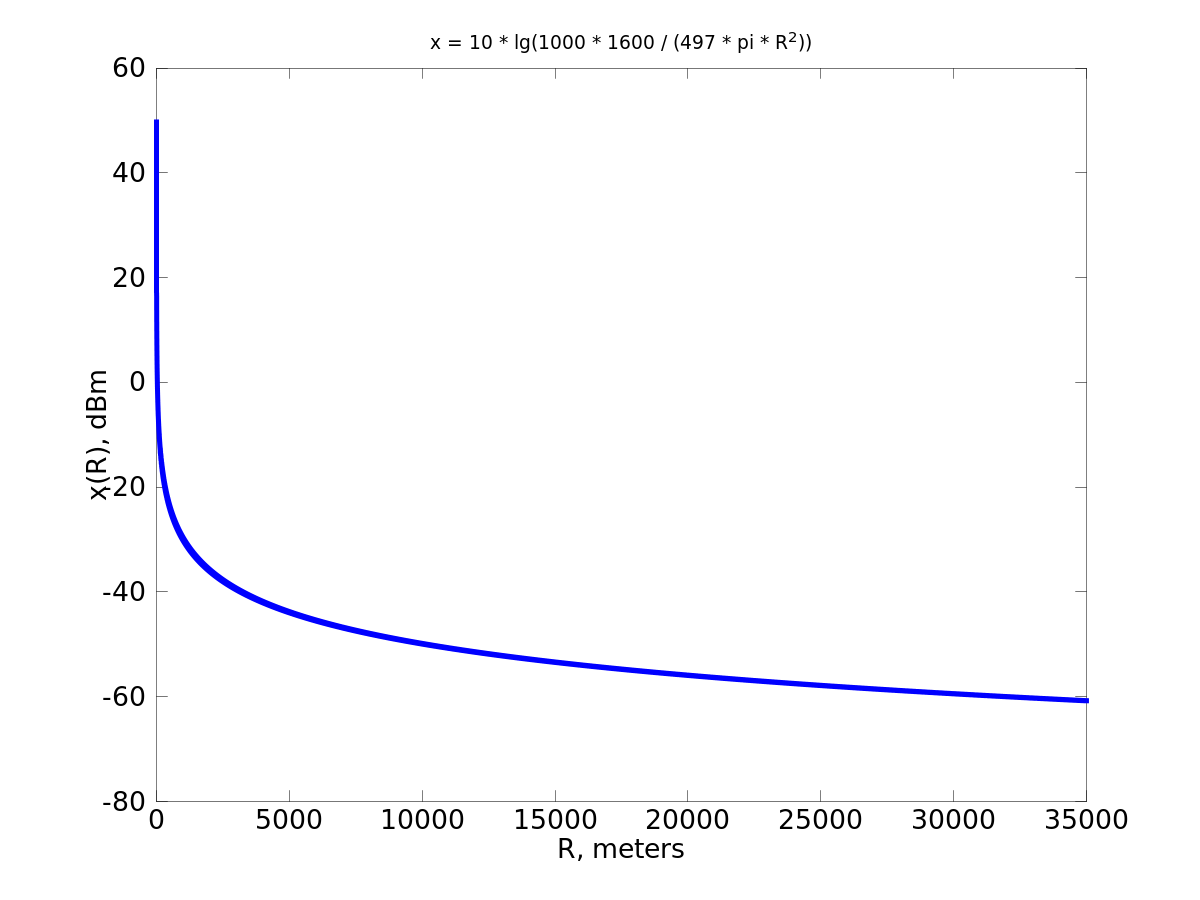
\includegraphics[width=1\linewidth]{bs40wdbm-contrast.png}\\
		Теоретически предсказанное затухание сигнала
		\column{0.5\textwidth}
		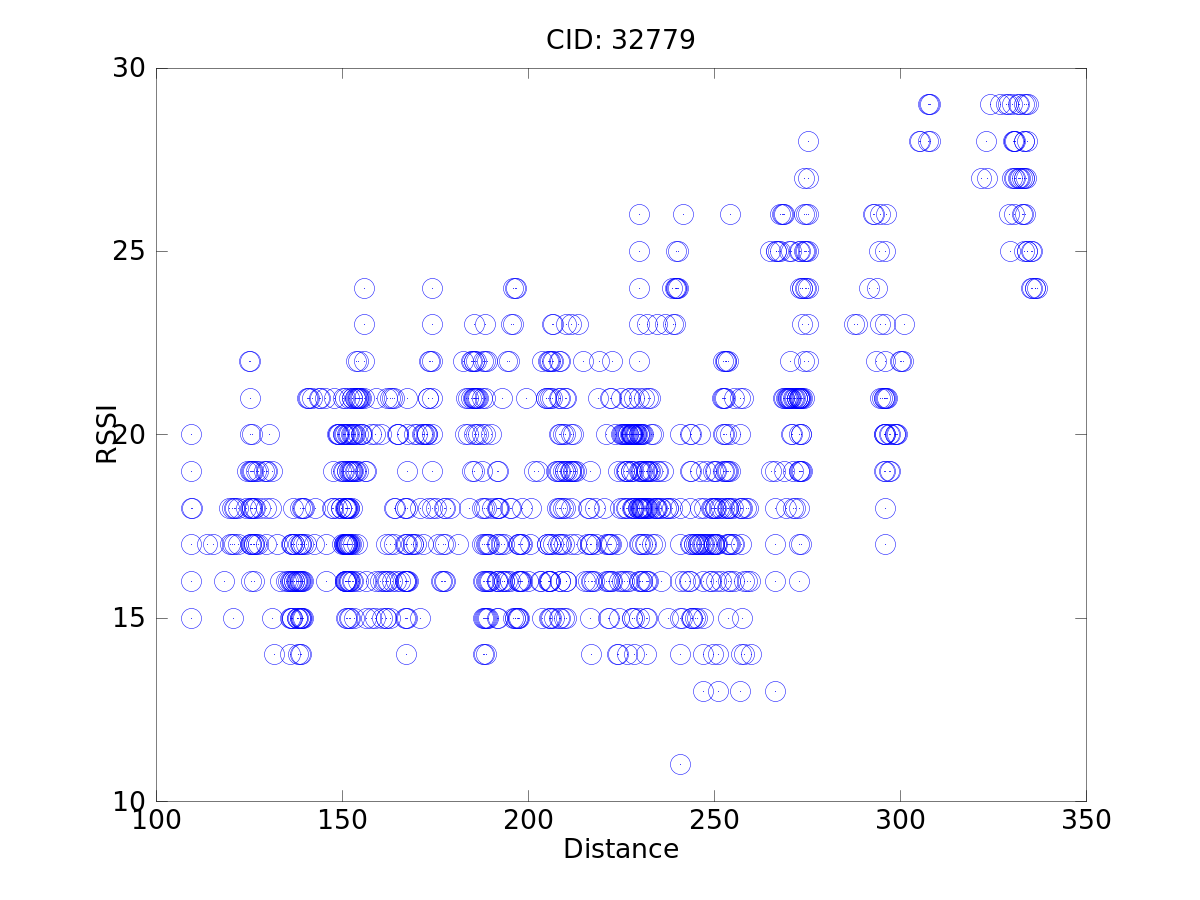
\includegraphics[width=1\linewidth]{cell32779raw-contrast.png}\\
		Реально принятые уровни
	\end{columns}
}

\frame{
	\frametitle{Общественный транспорт}
	Заранее известный маршрут:
	\begin{itemize}
		\item
			Делает задачу одномерной
		\item
			Позволяет набрать больше статистики
	\end{itemize}
}

\frame{
	\frametitle{Статистические методы}
	\begin{tabular}{|p{0.4\textwidth}|p{0.25\textwidth}|p{0.25\textwidth}|}
		\hline
		{\bf{}Параметр} & {\bf{}Расстояние Махаланобиса} & {\bf{}Байесовский классификатор} \\
		\hline
		Непрерывность аргумента & - & - \\
		\hline
		Непрерывность значения & + & - \\
		\hline
		Устойчивость к выбросам & - & + \\
		\hline
	\end{tabular}
}

\frame{
	\frametitle{Предлагаемый алгоритм}
	И был создан новый алгоритм, который:
	\begin{enumerate}
		\item
			Учитывает непрерывность случайной переменной --- уровня сигнала;
		\item
			Учитывает значения в соседних точках;
		\item
			Устойчив к выбросам.
	\end{enumerate}
	Как он работает?
}

\frame{
	\frametitle{Выборка из базы}
	\begin{columns}[T]
		\begin{column}{0.75\textwidth}
			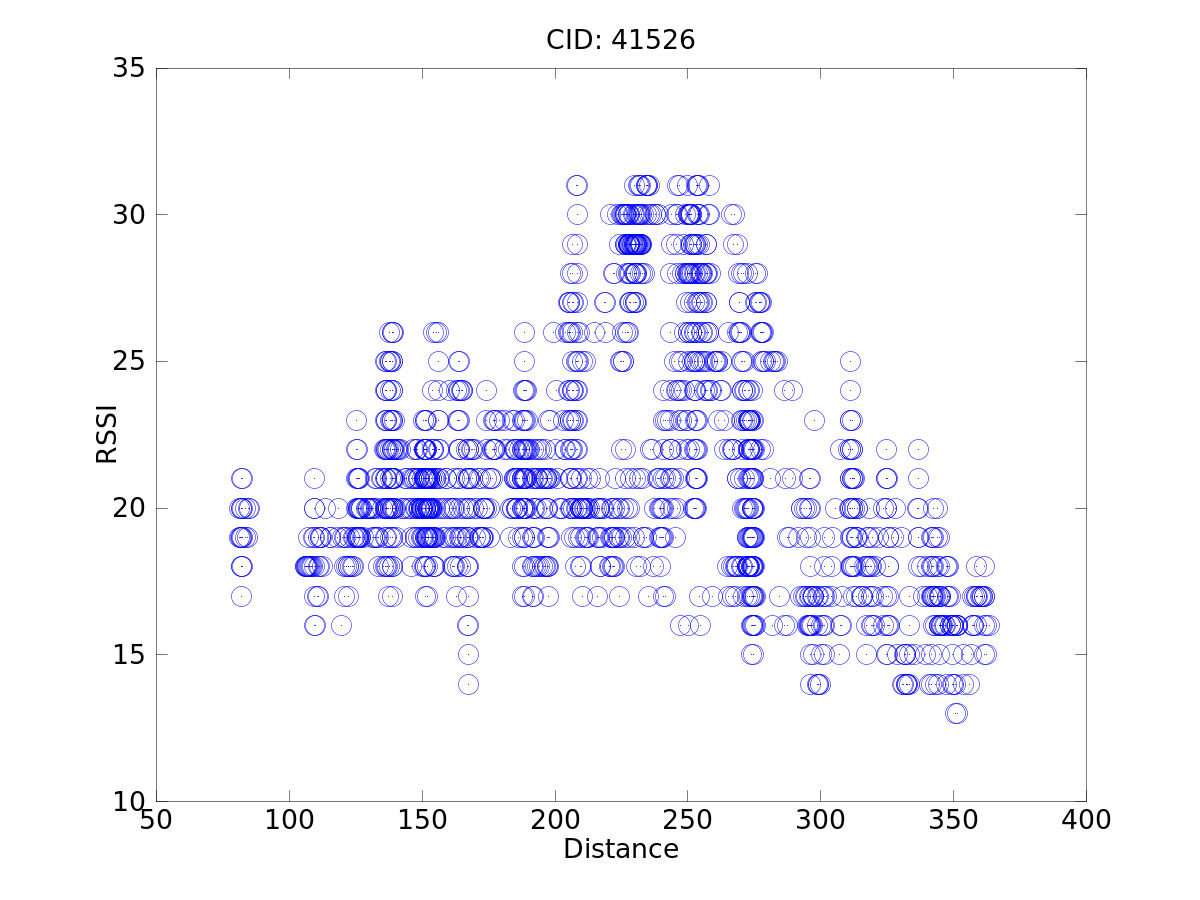
\includegraphics[width=0.9\textwidth]{cell41526raw-contrast.png}

			\hspace{1em}
			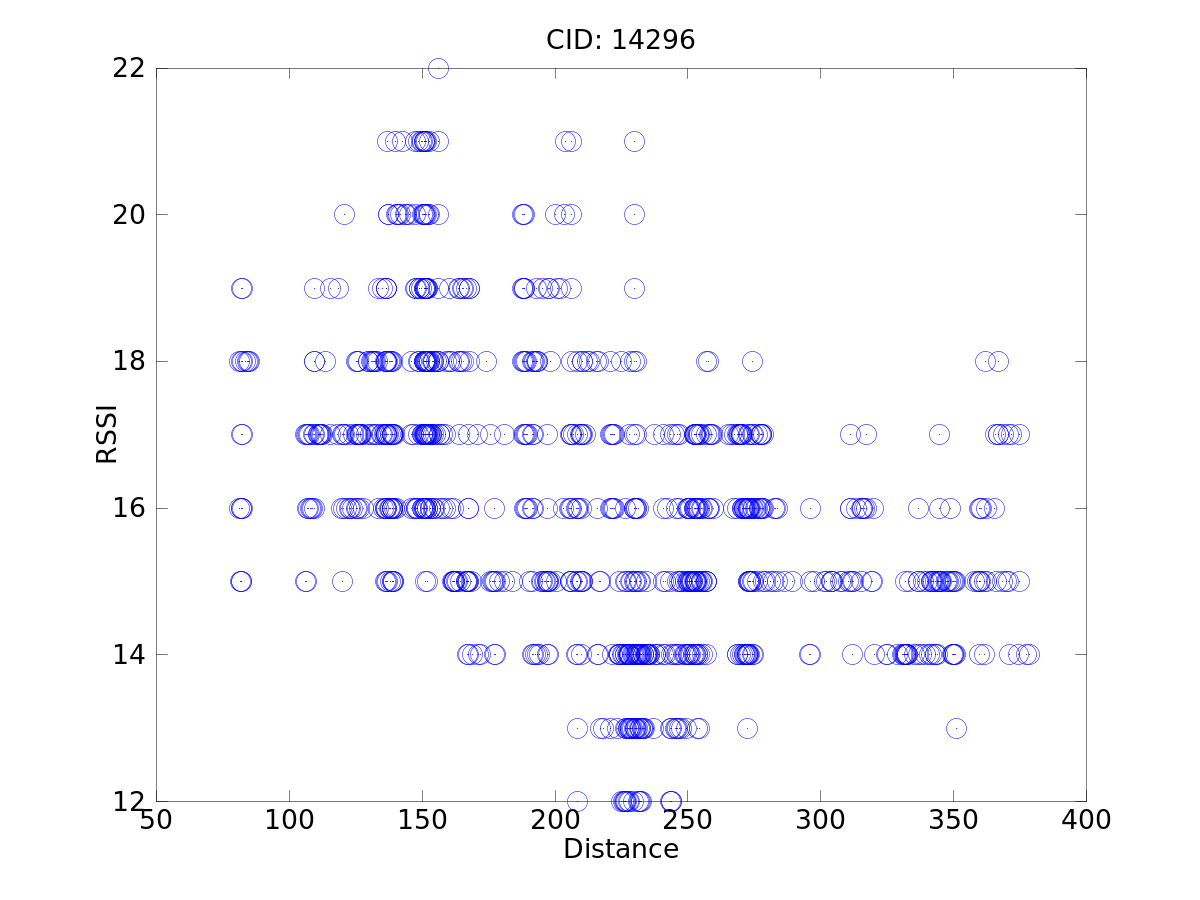
\includegraphics[width=0.37\textwidth]{cell14296raw-contrast.png}
			\hspace{1em}
			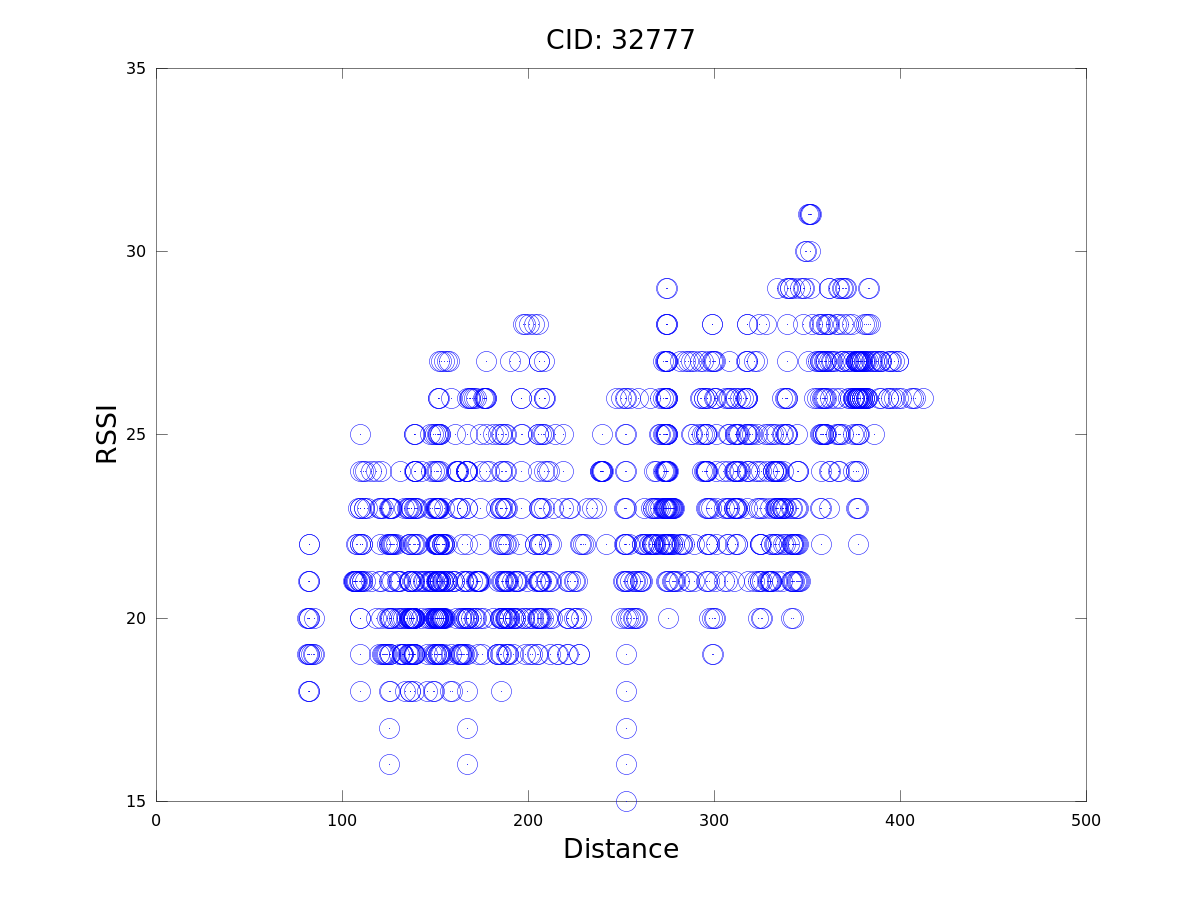
\includegraphics[width=0.37\textwidth]{cell32777raw-contrast.png}
			\end{column}

		\begin{column}{0.32\textwidth}
			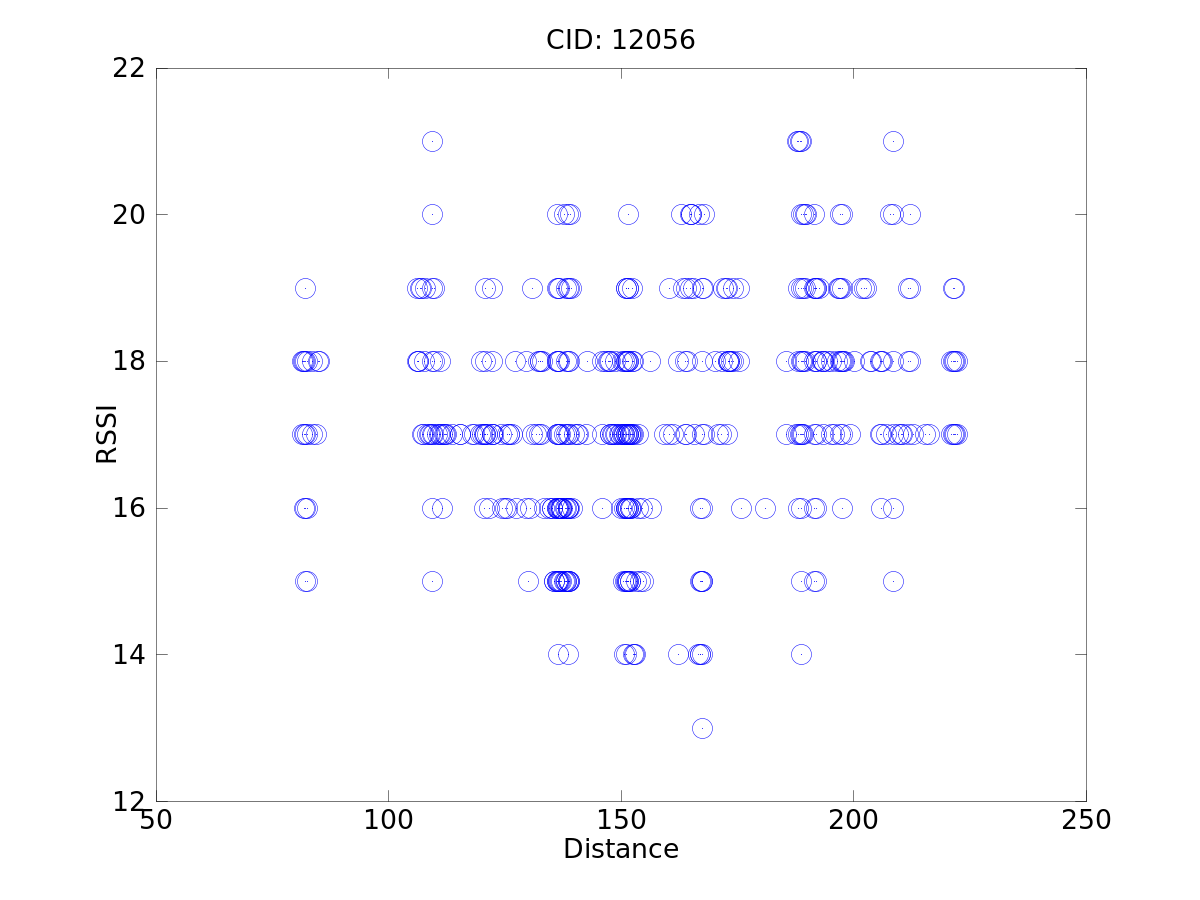
\includegraphics[width=0.95\textwidth]{cell12056raw-contrast.png}

			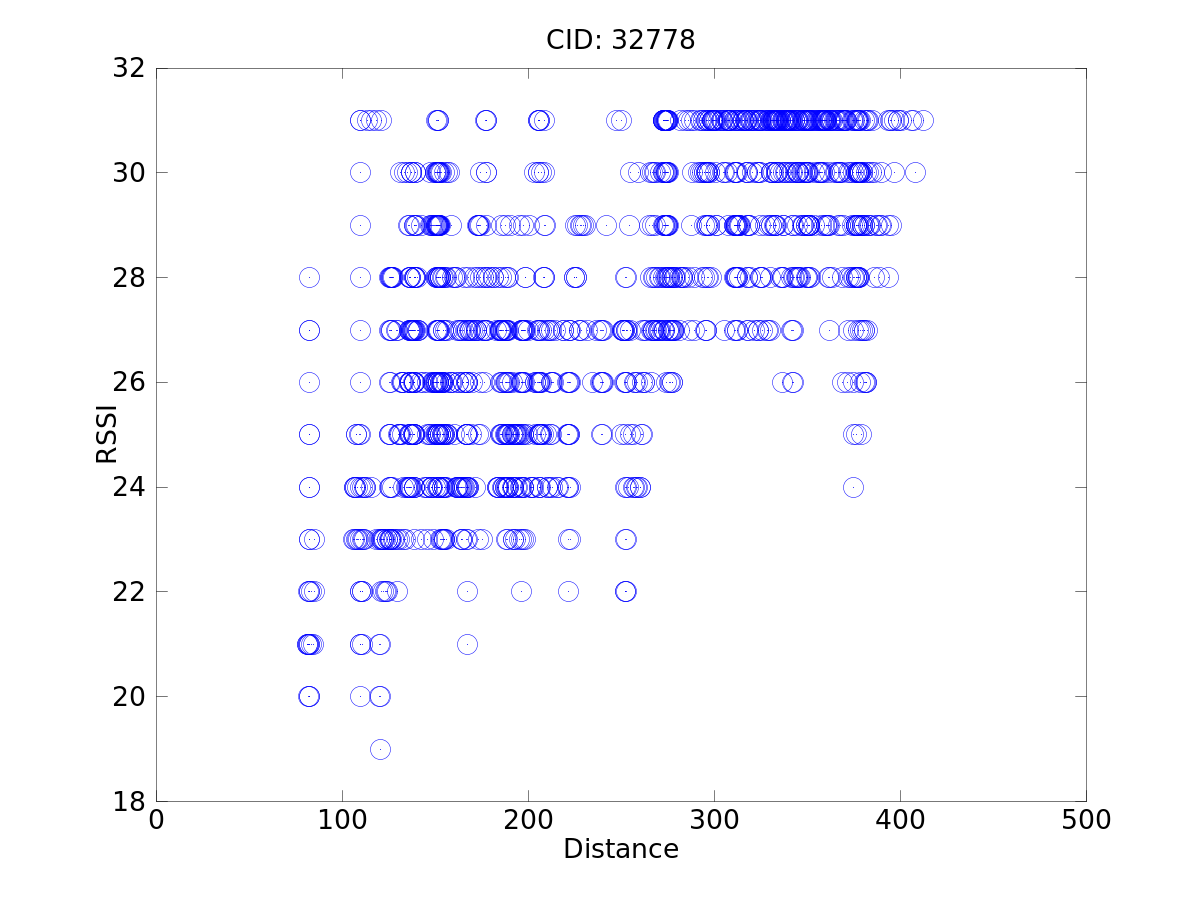
\includegraphics[width=0.95\textwidth]{cell32778raw-contrast.png}
	
			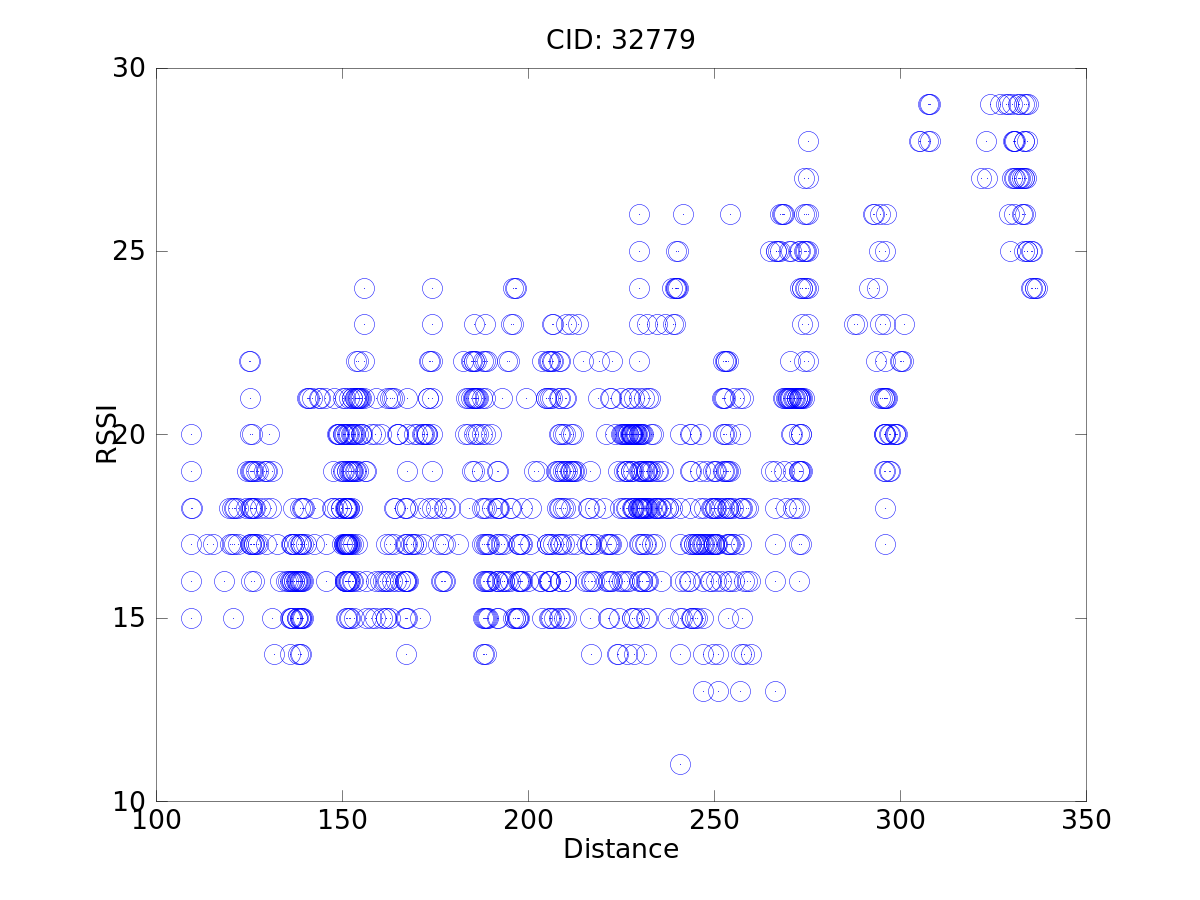
\includegraphics[width=0.95\textwidth]{cell32779raw-contrast.png}
		\end{column}
	\end{columns}
}

\frame{
	\frametitle{Интерполяция}
	\begin{columns}[T]
		\begin{column}{0.75\textwidth}
			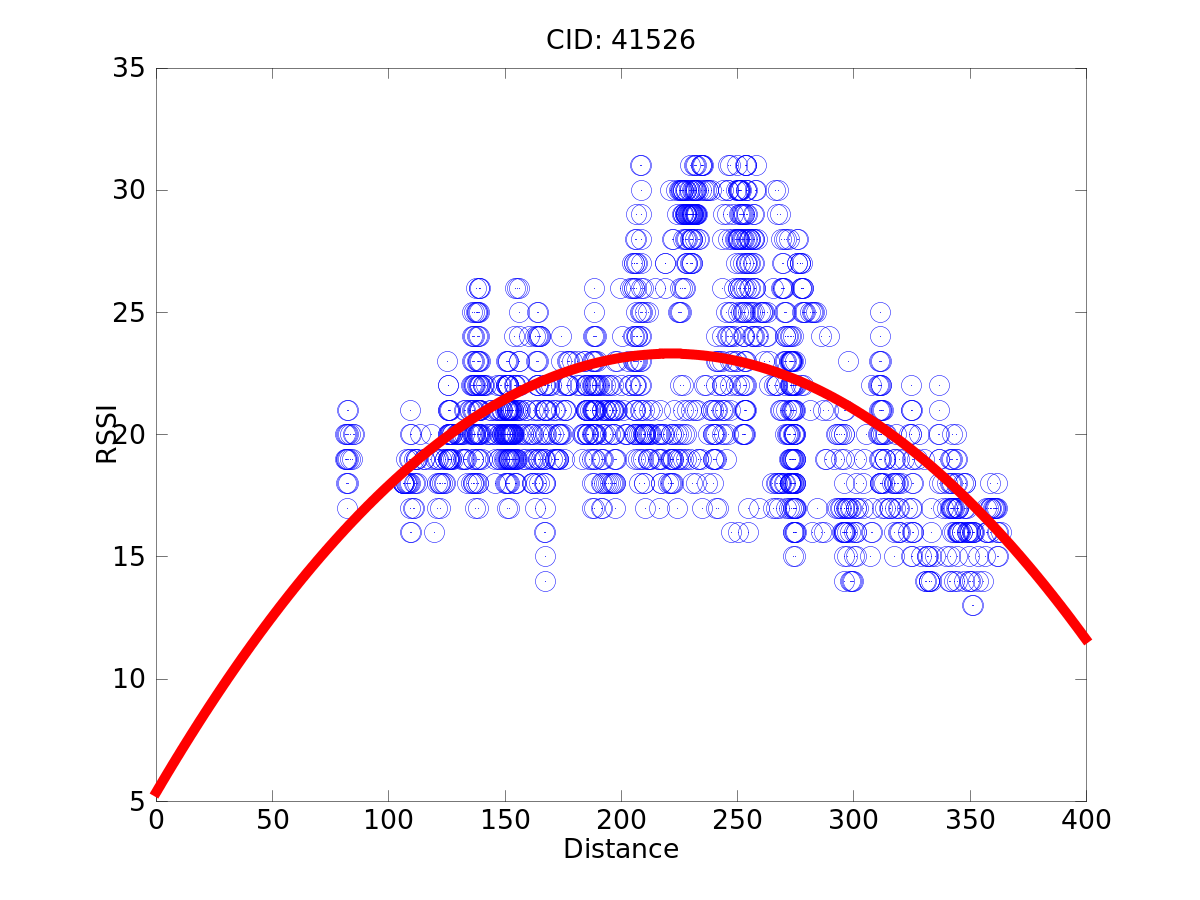
\includegraphics[width=0.9\textwidth]{cell41526inter-contrast.png}

			\hspace{1em}
			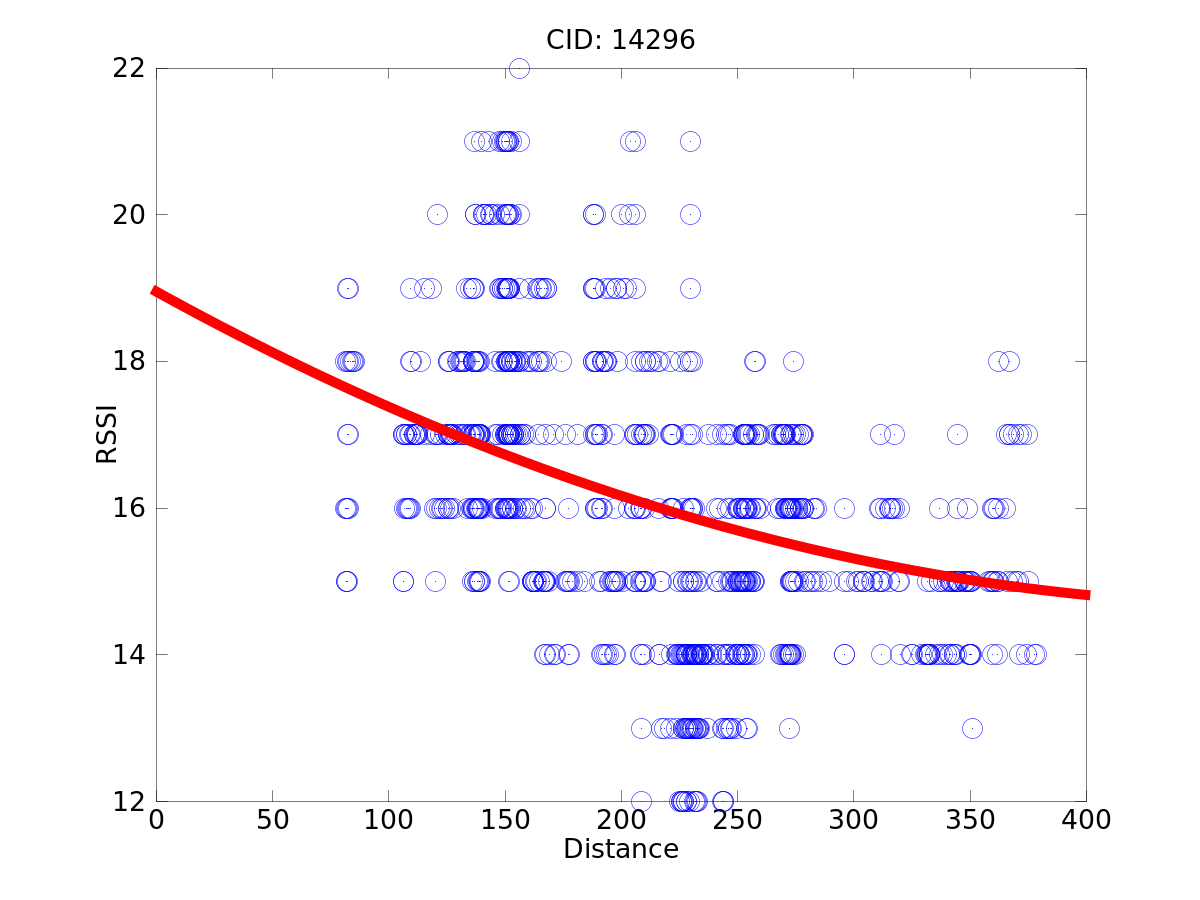
\includegraphics[width=0.37\textwidth]{cell14296inter-contrast.png}
			\hspace{1em}
			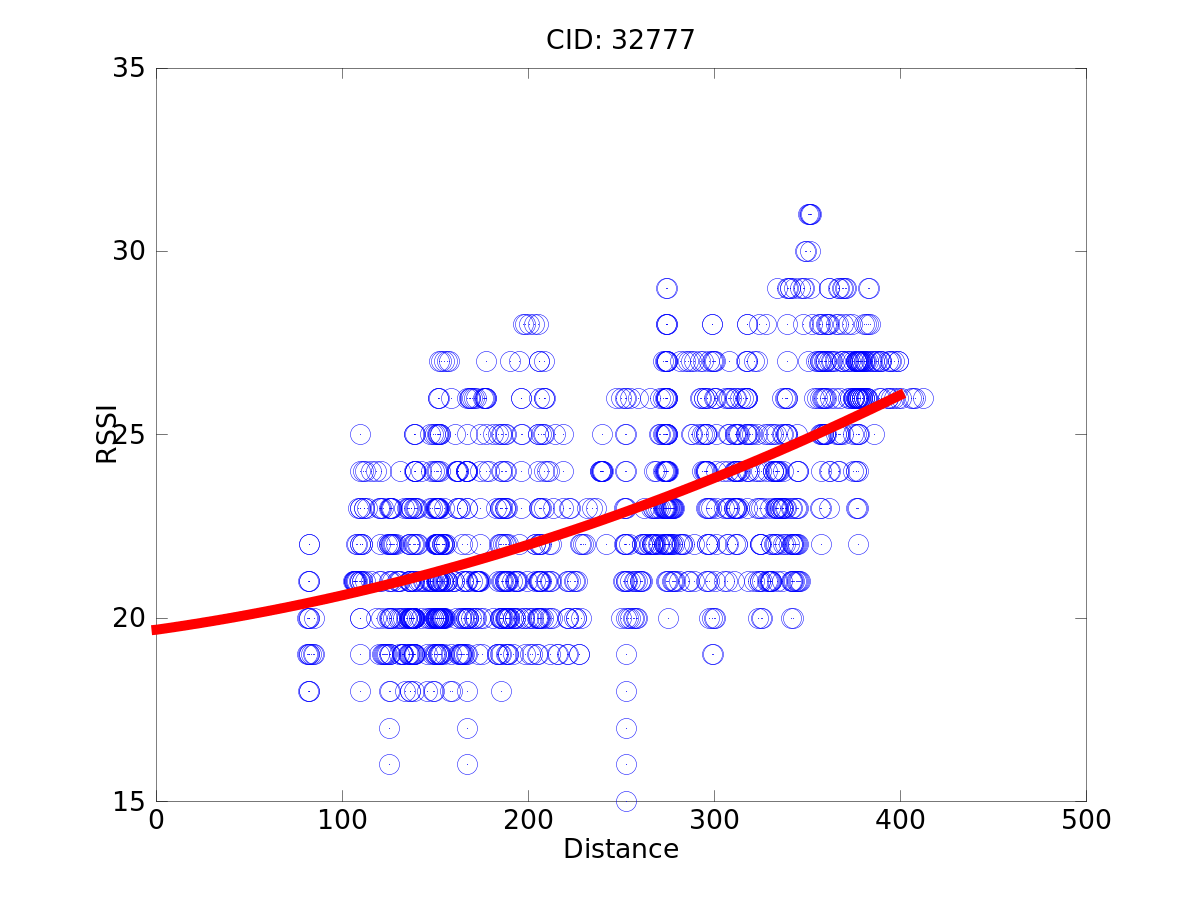
\includegraphics[width=0.37\textwidth]{cell32777inter-contrast.png}
			\end{column}

		\begin{column}{0.32\textwidth}
			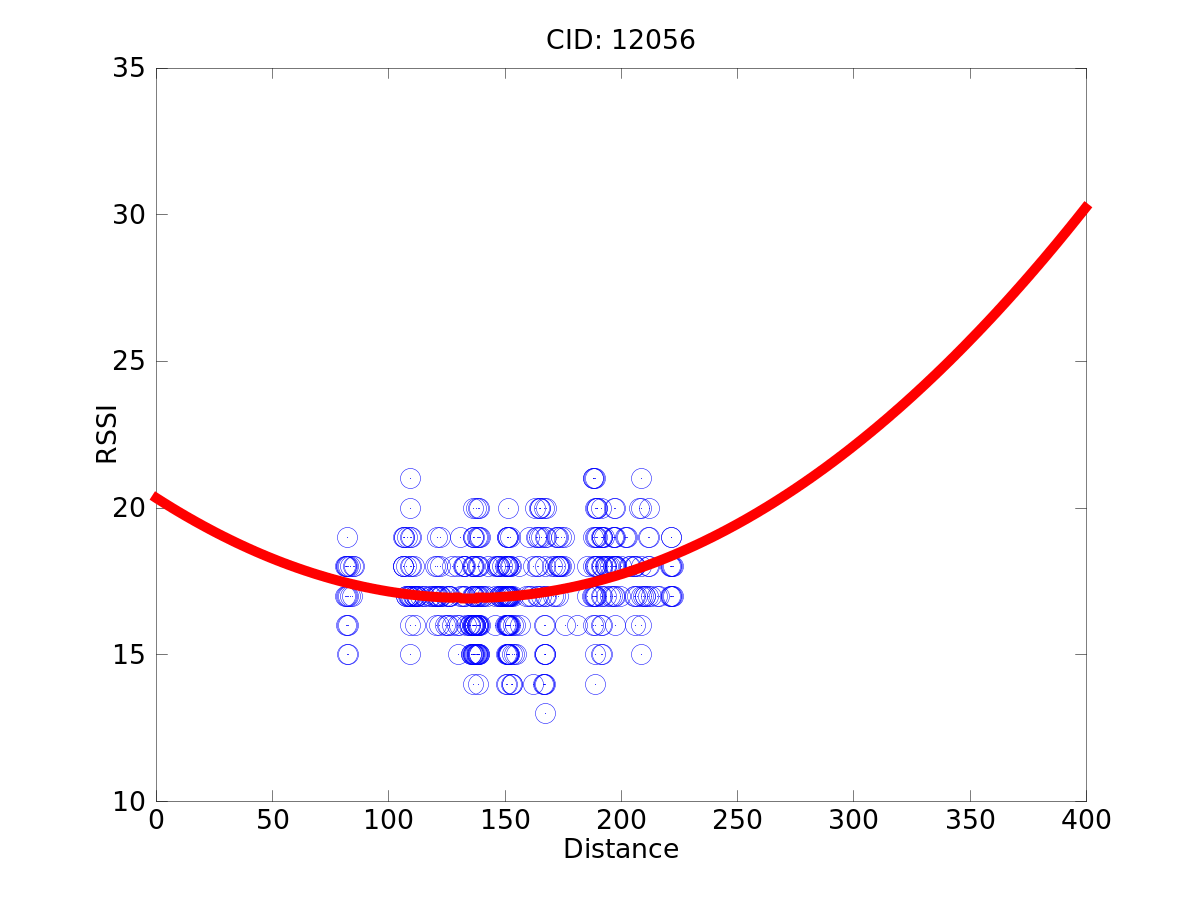
\includegraphics[width=0.95\textwidth]{cell12056inter-contrast.png}

			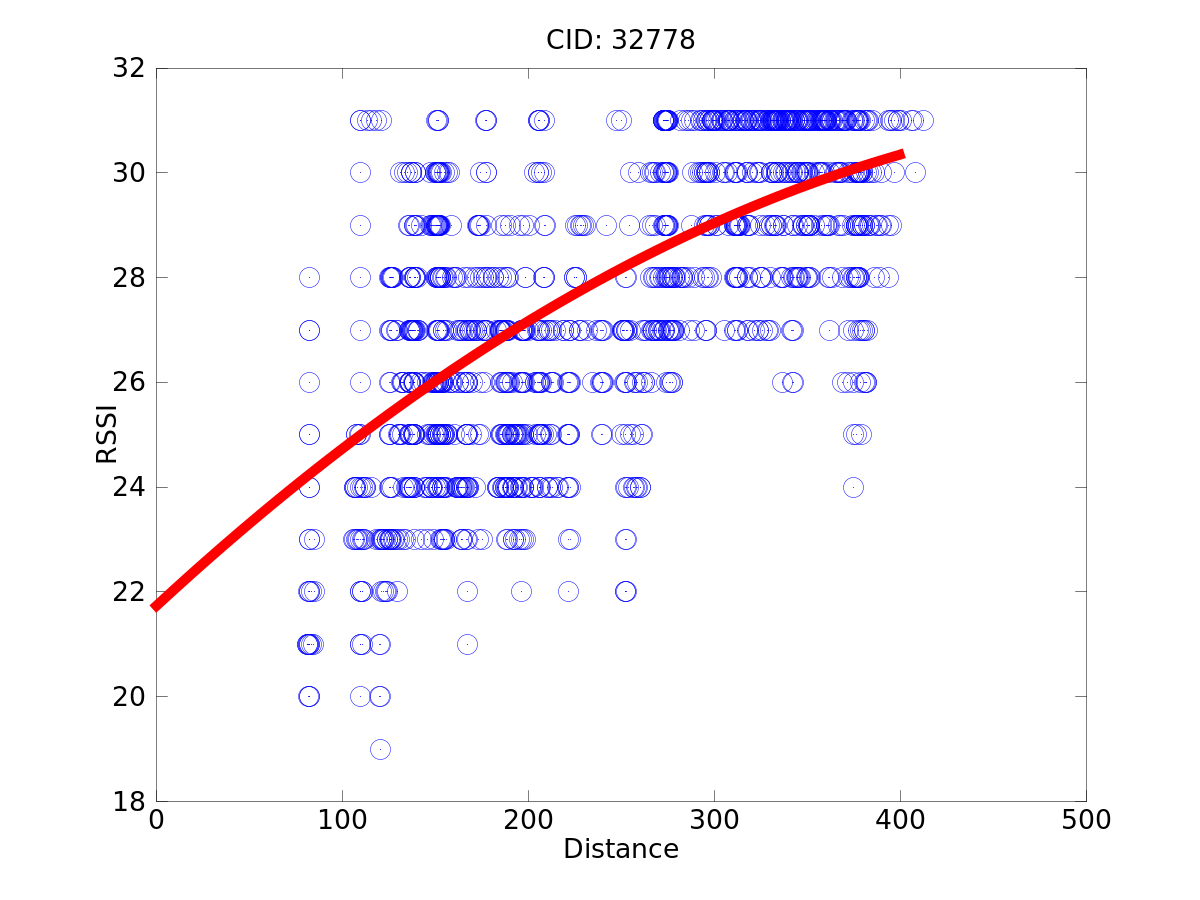
\includegraphics[width=0.95\textwidth]{cell32778inter-contrast.png}
	
			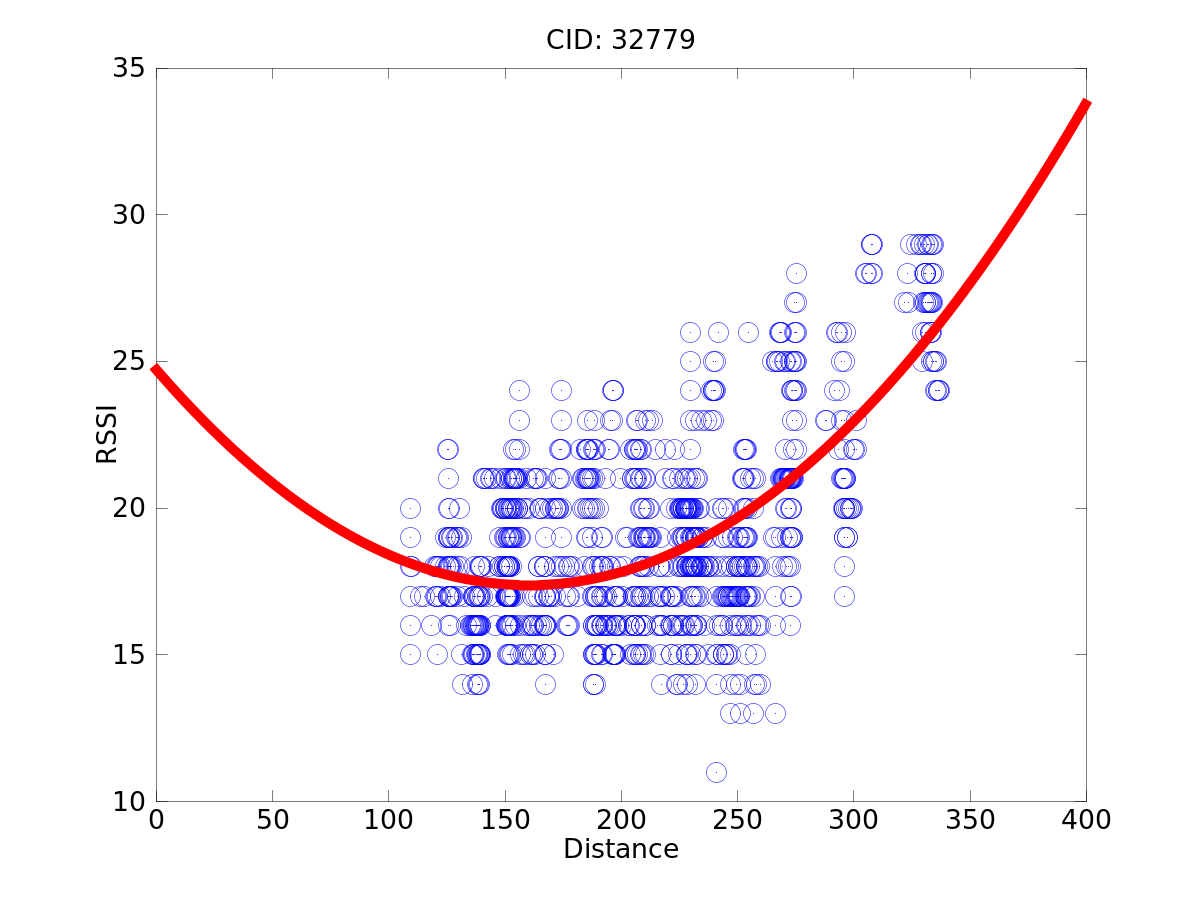
\includegraphics[width=0.95\textwidth]{cell32779inter-contrast.png}
		\end{column}
	\end{columns}

}

\frame{
	\frametitle{Псевдоплотность вероятности}
	Требования:
	\begin{enumerate}
		\item
			$\forall_{f(x), y}P(f(x), y)\in(0,1]$
		\item
			$\forall_{f(x), y}f(x) = y\Leftrightarrow{}P(f(x),y) = 1$
		\item
			$\lim\limits_{|f(x)-y|\to\infty}P(f(x),y) = 0$
	\end{enumerate}
	Вид:
	\begin{equation}
		P(f(x), y) = \frac{1}{1+(f(x)-y)^2}
		\nonumber
		\label{eq:pseudop}
	\end{equation}
}
\frame{
	\frametitle{Вычисление псевдоплотности}
	\begin{columns}[T]
		\begin{column}{0.75\textwidth}
			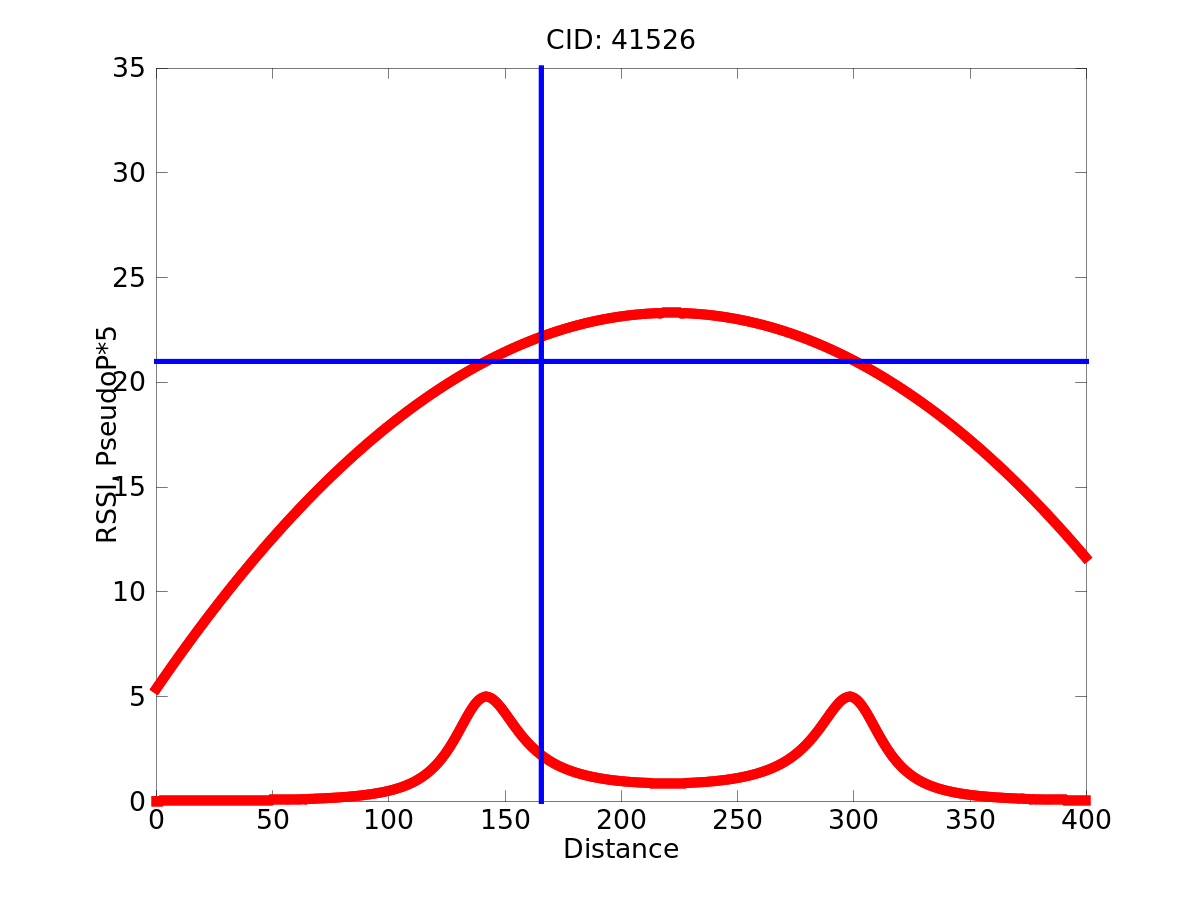
\includegraphics[width=0.9\textwidth]{cell41526pseudop-contrast.png}

			\hspace{1em}
			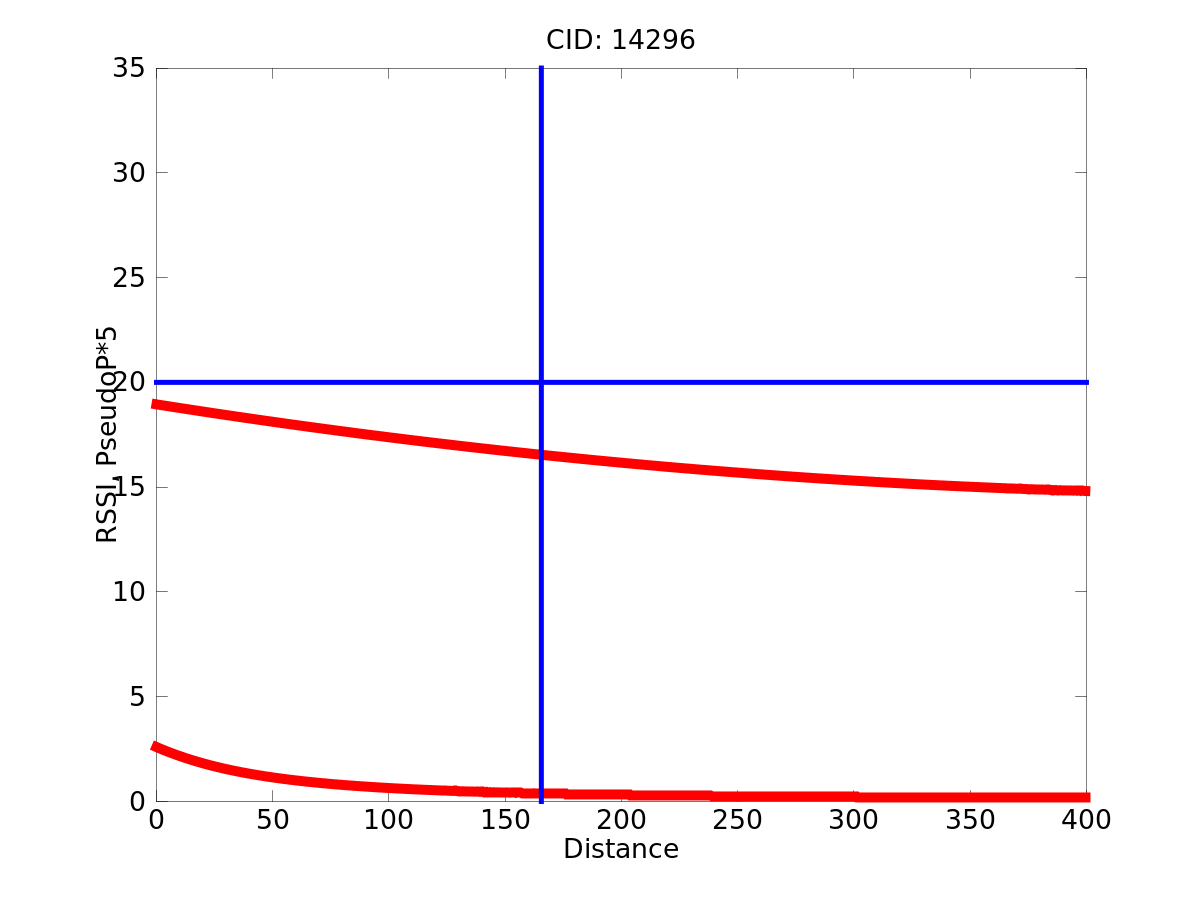
\includegraphics[width=0.37\textwidth]{cell14296pseudop-contrast.png}
			\hspace{1em}
			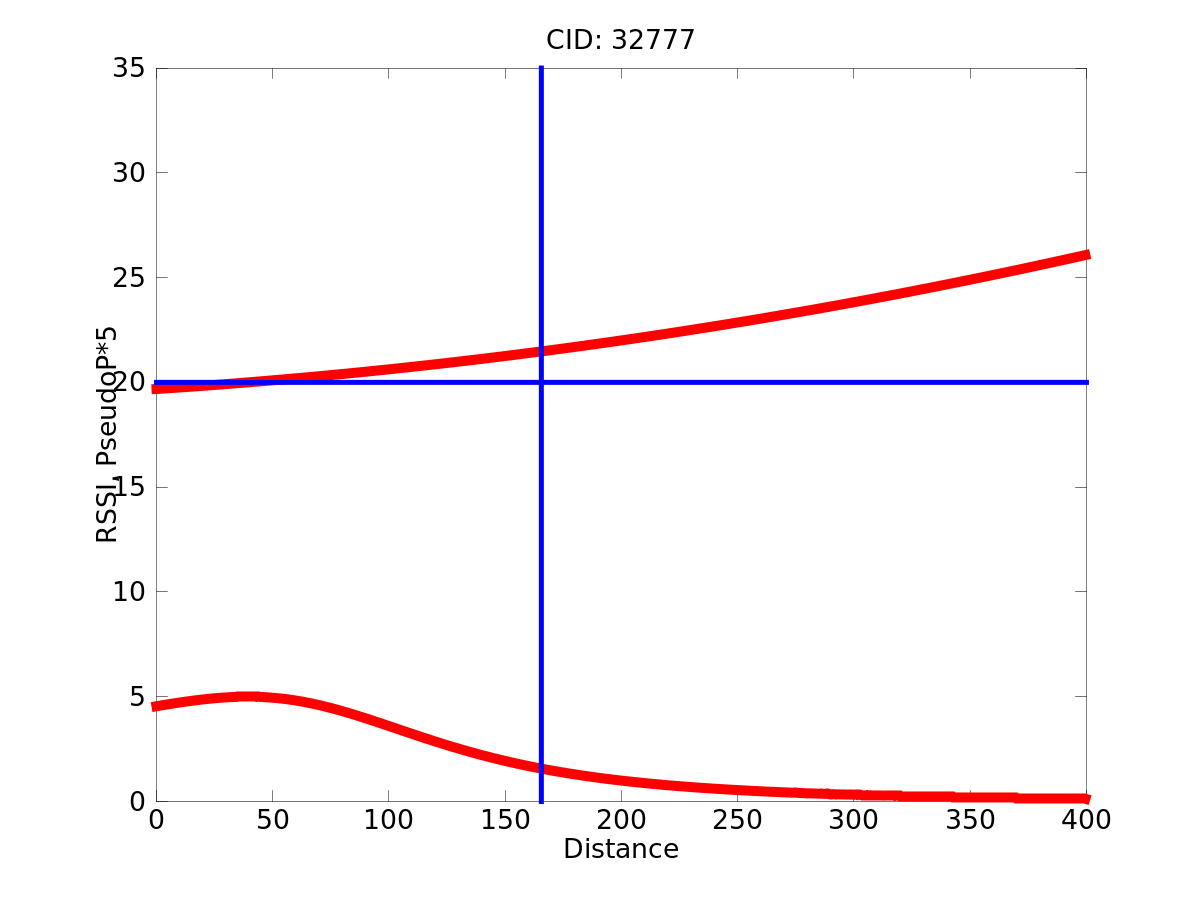
\includegraphics[width=0.37\textwidth]{cell32777pseudop-contrast.png}
			\end{column}

		\begin{column}{0.32\textwidth}
			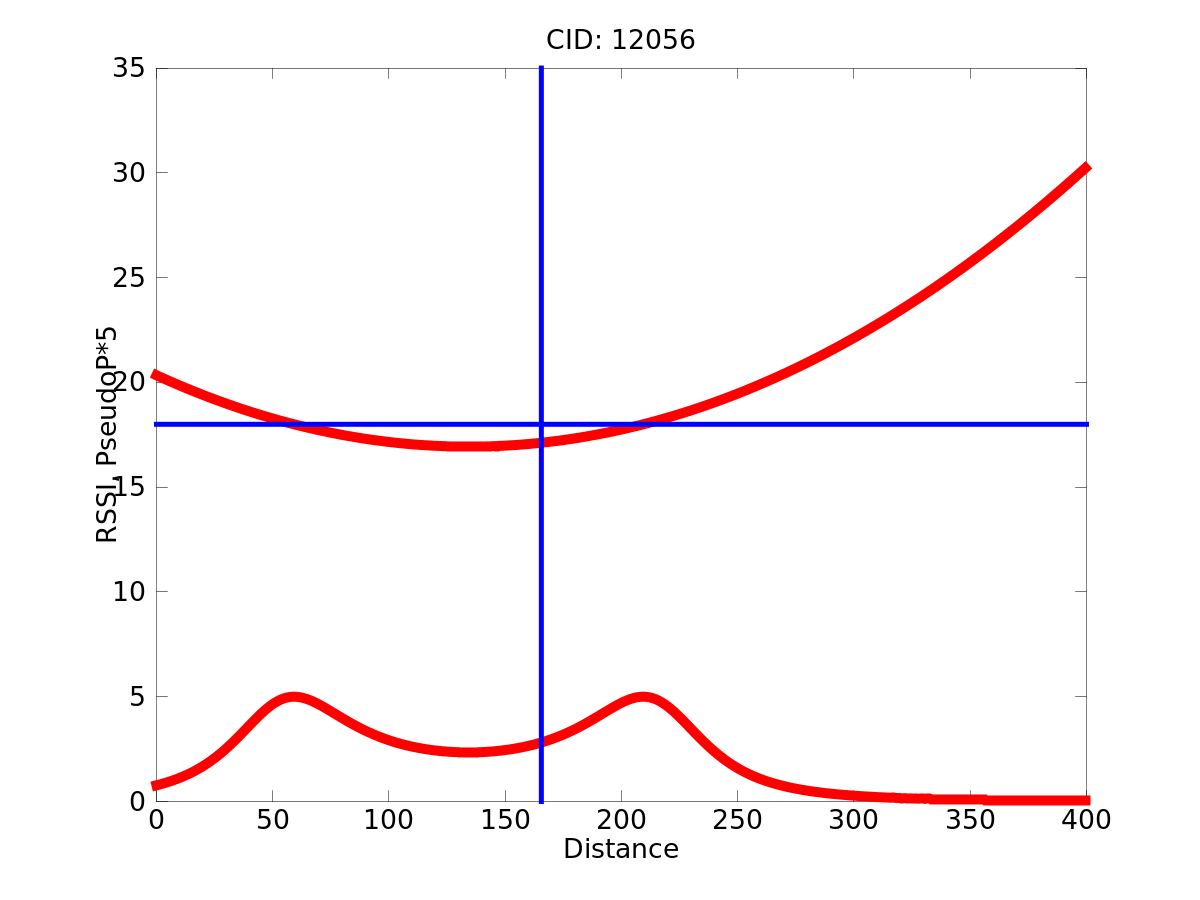
\includegraphics[width=0.95\textwidth]{cell12056pseudop-contrast.png}

			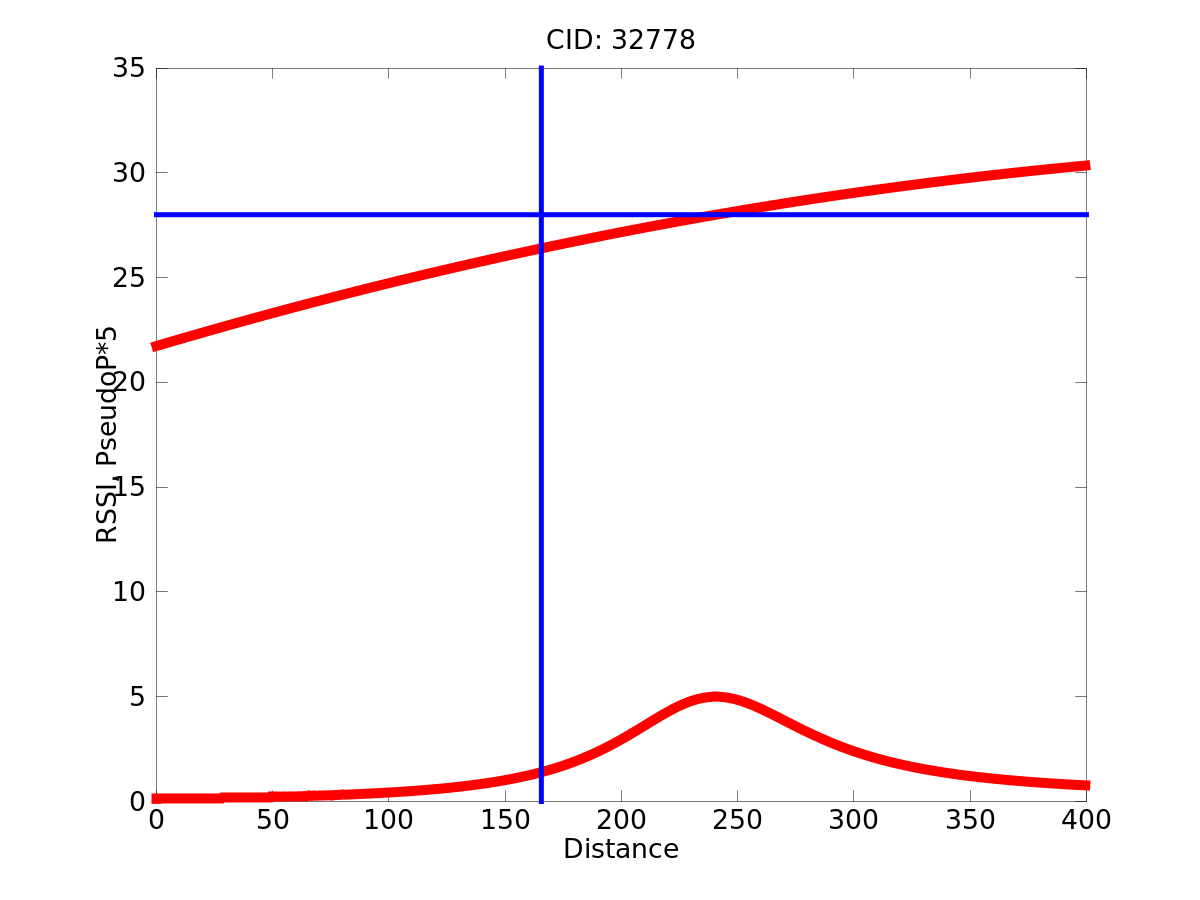
\includegraphics[width=0.95\textwidth]{cell32778pseudop-contrast.png}
	
			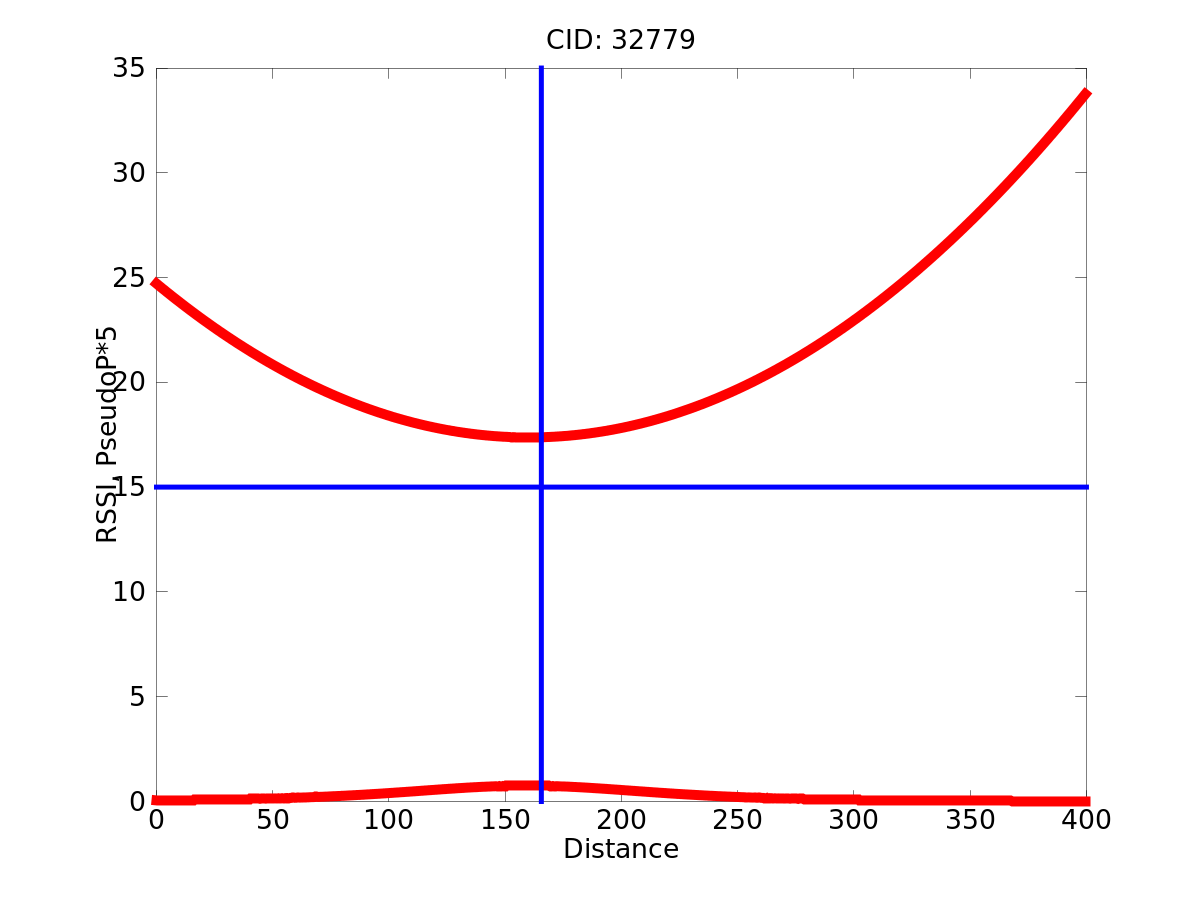
\includegraphics[width=0.95\textwidth]{cell32779pseudop-contrast.png}
		\end{column}
	\end{columns}

}

\frame{
	\frametitle{Итоговая псевдоплотность}
	Результат: 143 метра, истина: 165,5 метров.

	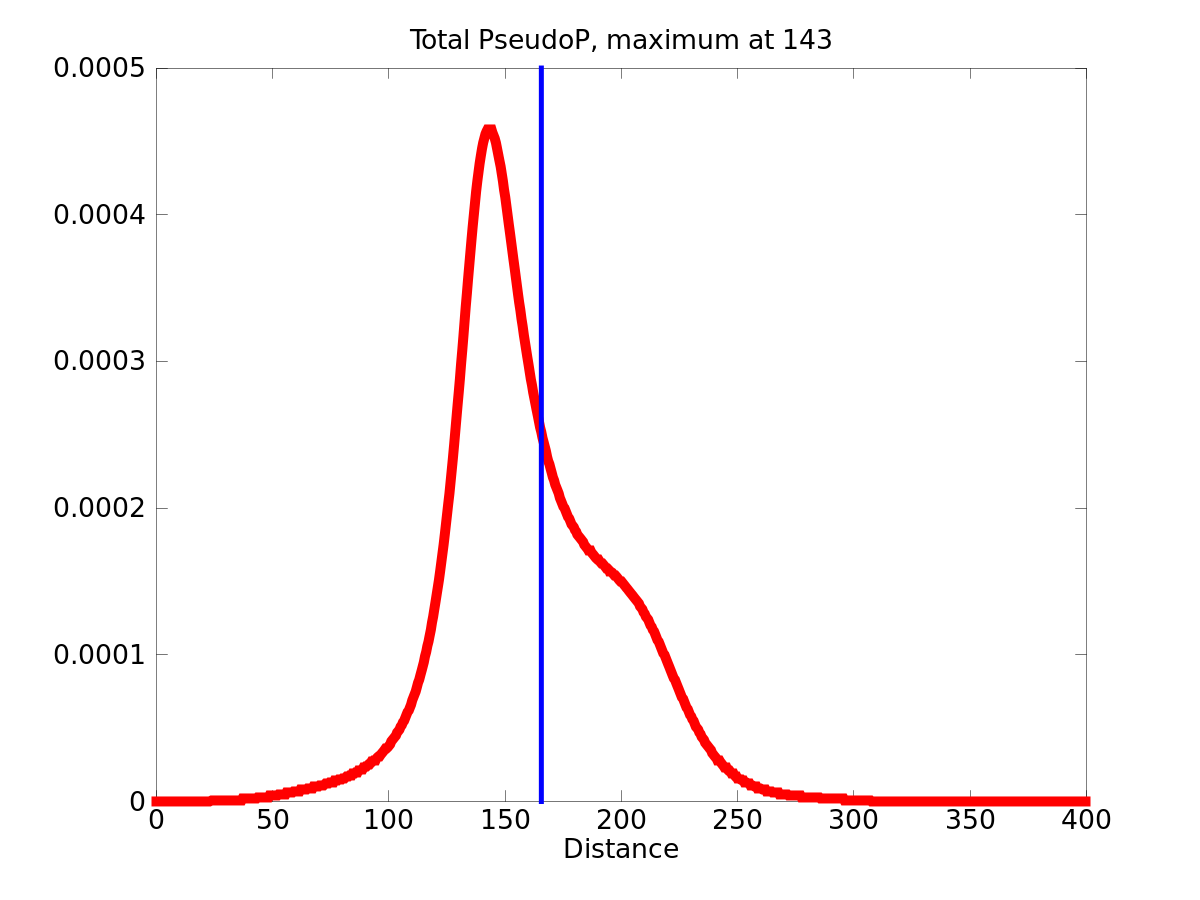
\includegraphics[height=0.8\textheight]{totalpseudop-contrast.png}
}

\frame{
	\frametitle{Архитектура системы}
	\centerline{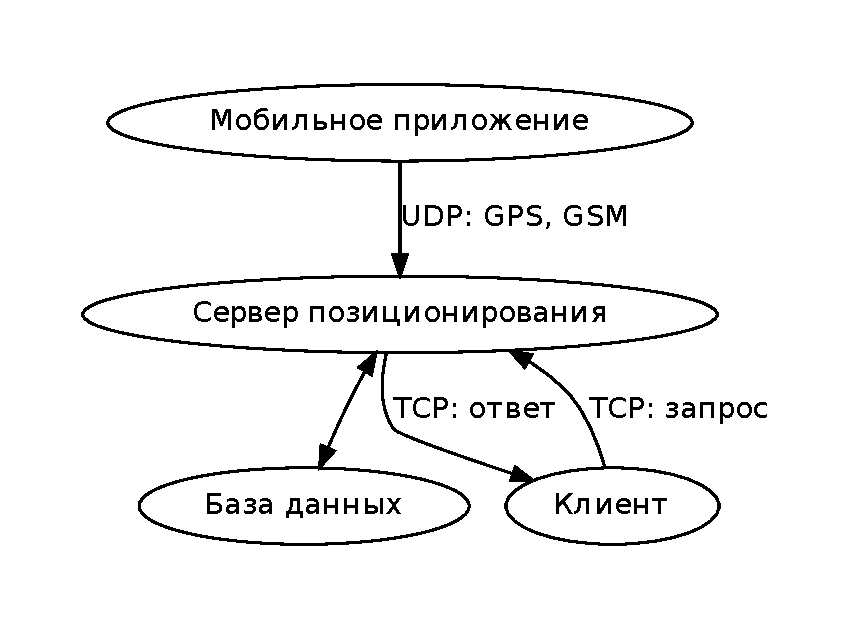
\includegraphics[height=0.8\textheight]{general-arch.pdf}}
}

\frame{
	\frametitle{Тестирование}
	\centerline{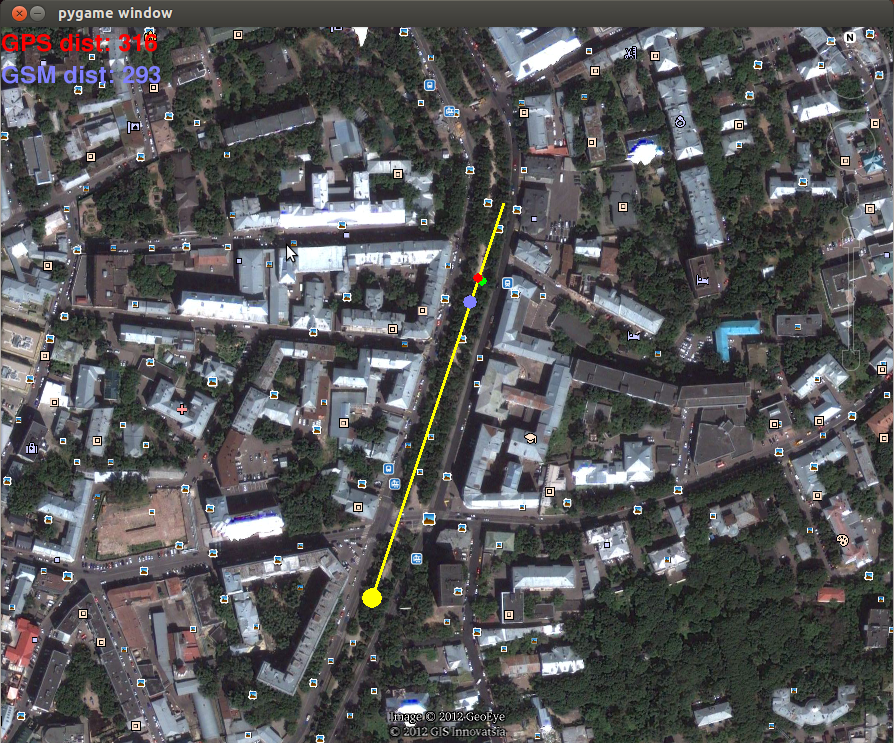
\includegraphics[height=0.8\textheight]{gfront-gsm-mode.png}}
}

\frame{
	\frametitle{Гистограмма ошибок}
	Опытов: 176, математическое ожидание ошибки: 49 метров.

	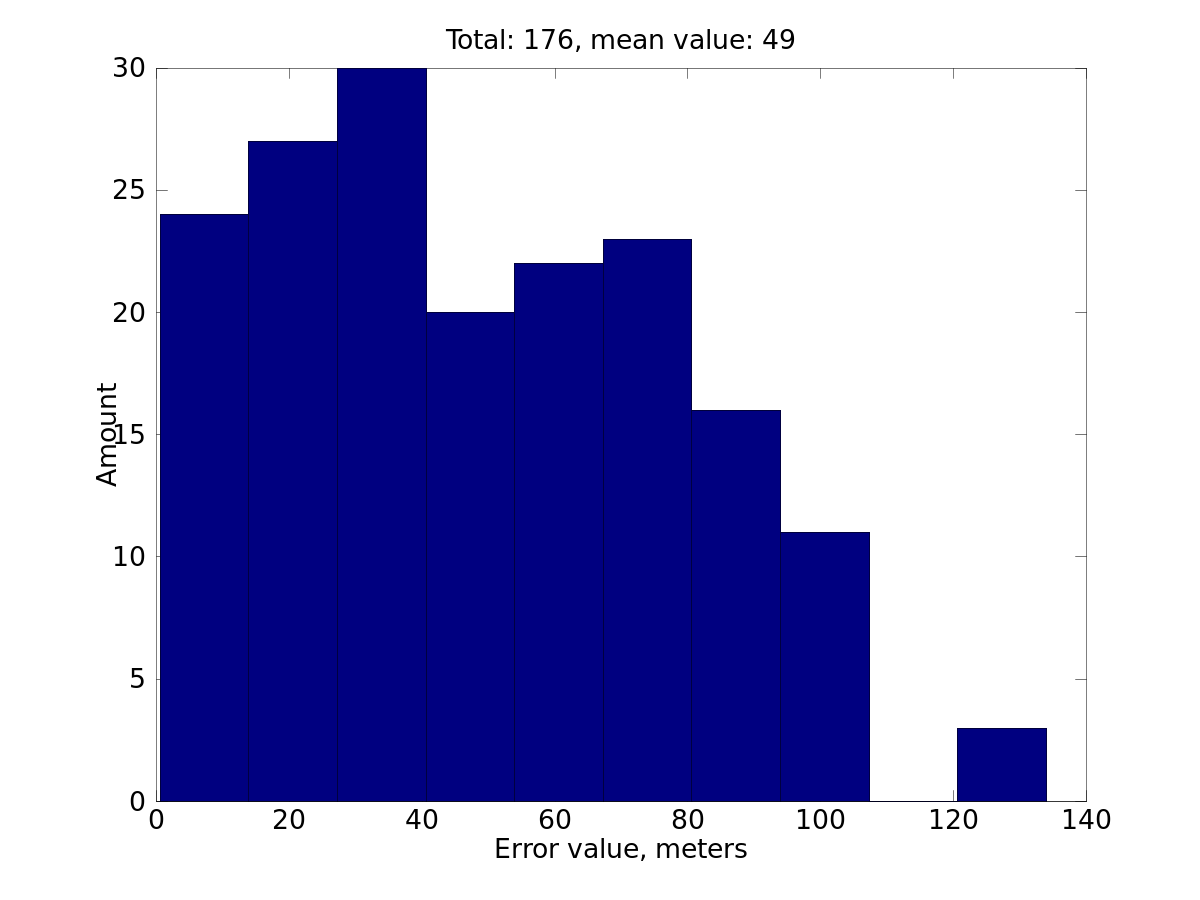
\includegraphics[height=0.8\textheight]{errhist-contrast.png}
}

\begin{frame}[fragile]
	\frametitle{Сравнение систем}
	\begin{tabular}{|p{0.2\textwidth}|p{0.2\textwidth}|p{0.23\textwidth}|p{0.2\textwidth}|}
		\hline
		{\bf{}Параметр} & {\bf{}GPS} & {\bf{}Триангуляция} & {\bf{}Созданная} \\
		\hline
		Точность, м & 10 & 200 & 50 \\
		\hline
		Стоимость & GPS+GSM & GSM & GSM \\
		\hline
		Покрытие & Земля & Город & Маршрут \\
		\hline
	\end{tabular}
\end{frame}

\frame{
	\frametitle{Исследование данных}
\begin{figure}[h]
	\begin{columns}[T]
		\column{0.45\textwidth}
			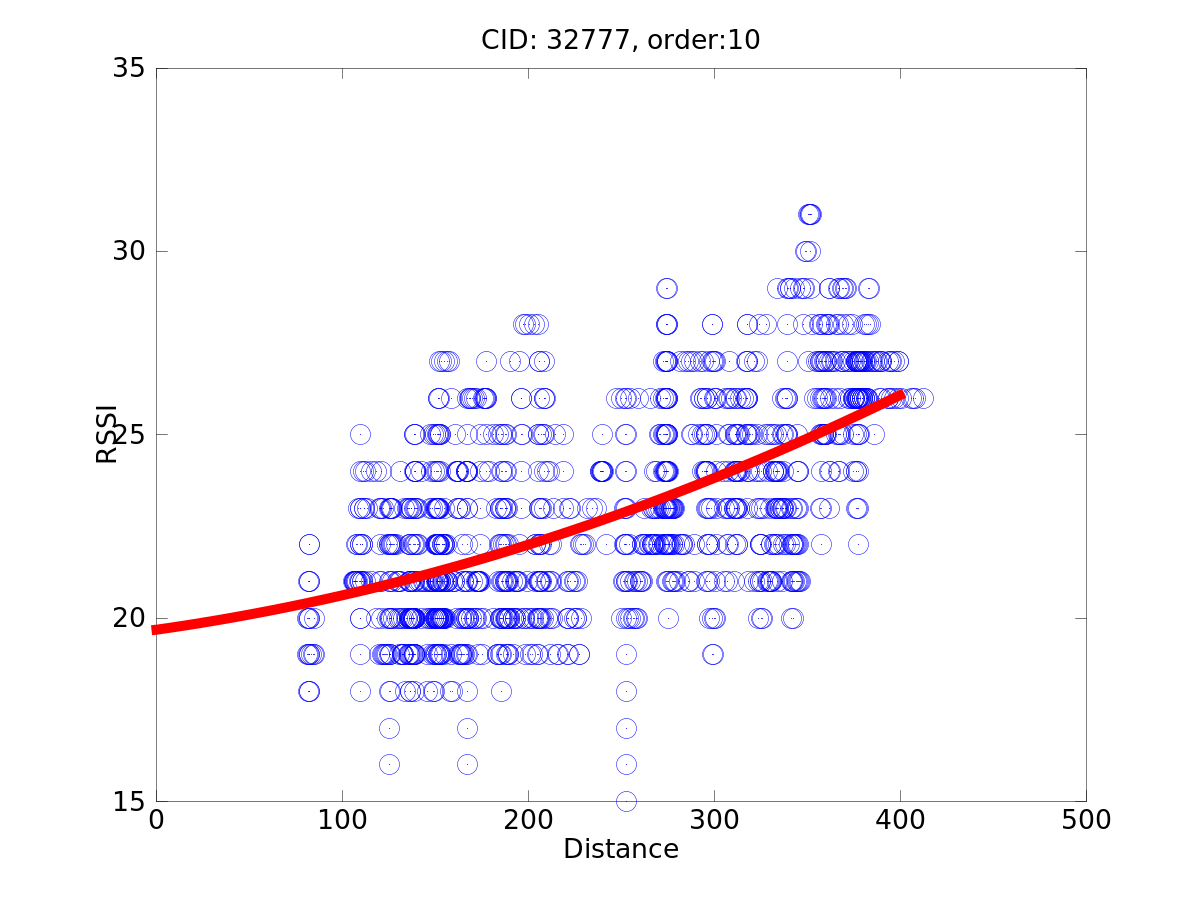
\includegraphics[width=1\textwidth]{cell32777inter10-contrast.png}

			Максимальная степень: 10
		\column{0.45\textwidth}
			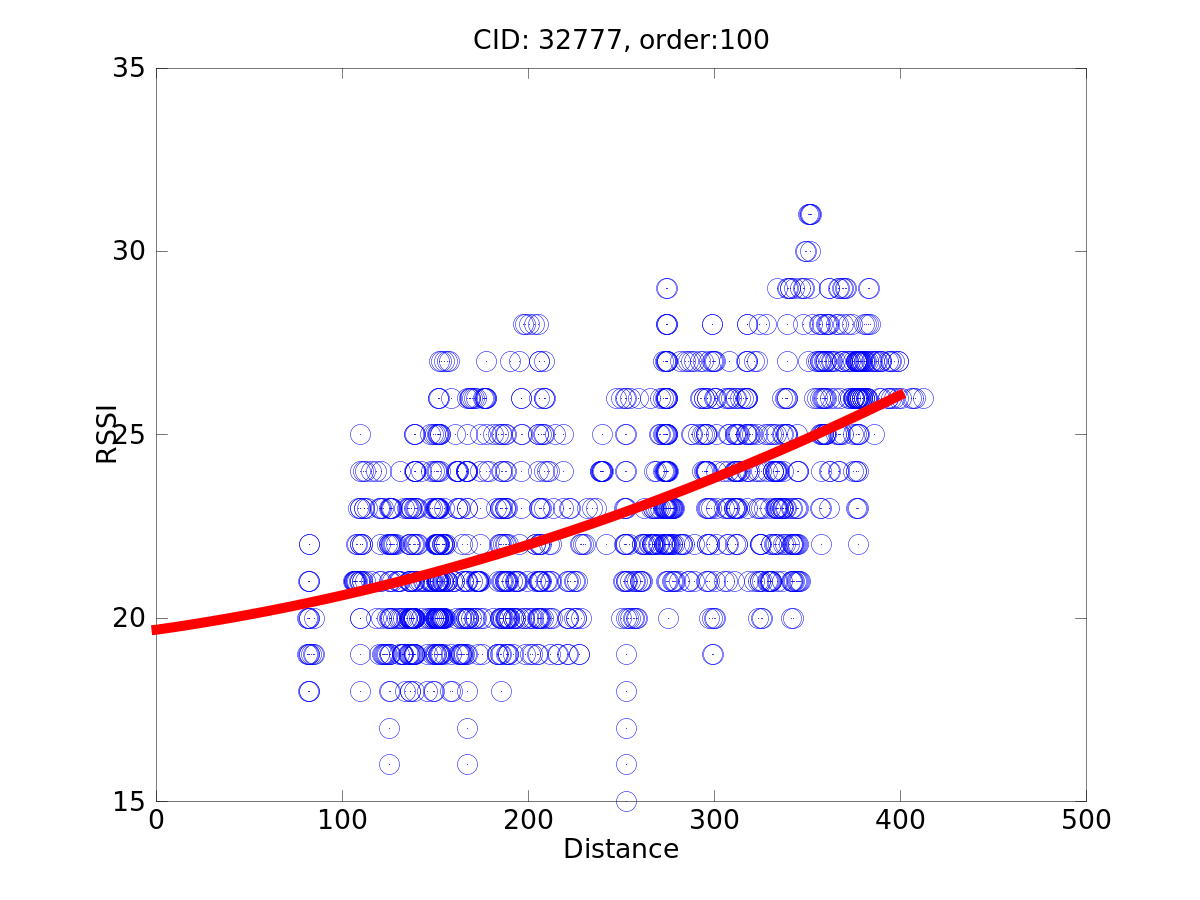
\includegraphics[width=1\textwidth]{cell32777inter100-contrast.png}
			
			Максимальная степень: 100
	\end{columns}
\end{figure}
}

\frame{
	\frametitle{Выводы}
	\begin{enumerate}
		\item
			Созданный метод работает;
		\item
			Точность лучше триангуляции;
		\item
			Точность не достигает GPS;
		\item
			Требуются дополнительные исследования.
	\end{enumerate}
}
\frame{\titlepage}

\appendix
\newcounter{finalframe}
\setcounter{finalframe}{\value{framenumber}}
\setbeamertemplate{footline}
{
  \leavevmode%
  \hbox{\large%
  \begin{beamercolorbox}[wd=.3\paperwidth,ht=2.25ex,dp=1ex,center]{author in head/foot}%
    \usebeamerfont{author in head/foot}\insertshortauthor
  \end{beamercolorbox}%
  \begin{beamercolorbox}[wd=.59\paperwidth,ht=2.25ex,dp=1ex,center]{title in head/foot}%
    \usebeamerfont{title in head/foot}\insertshorttitle
  \end{beamercolorbox}%
  \begin{beamercolorbox}[wd=.11\paperwidth,ht=2.25ex,dp=1ex,right]{date in head/foot}%
	\insertframenumber\hspace*{2ex}
  \end{beamercolorbox}}%
  \vskip0pt%
}

\frame{
	\frametitle{Потоки сервера}
	\centerline{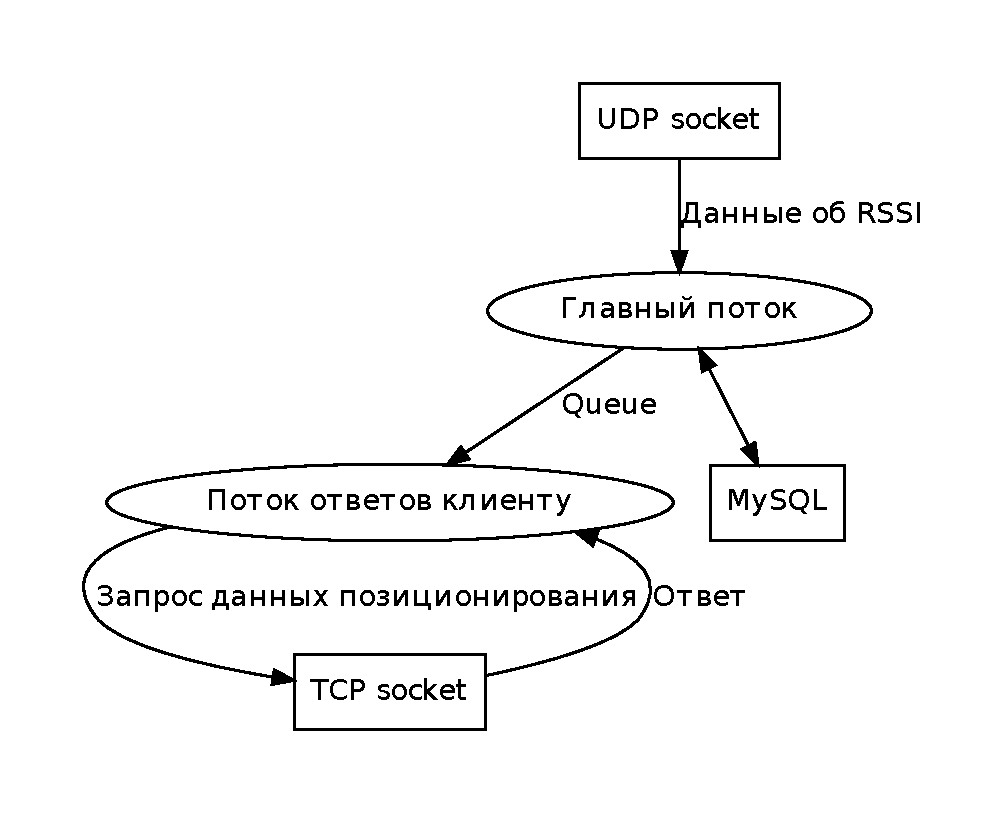
\includegraphics[height=0.8\textheight]{server-threads.pdf}}
}

\frame{
	\frametitle{Режим сбора данных}
	\centerline{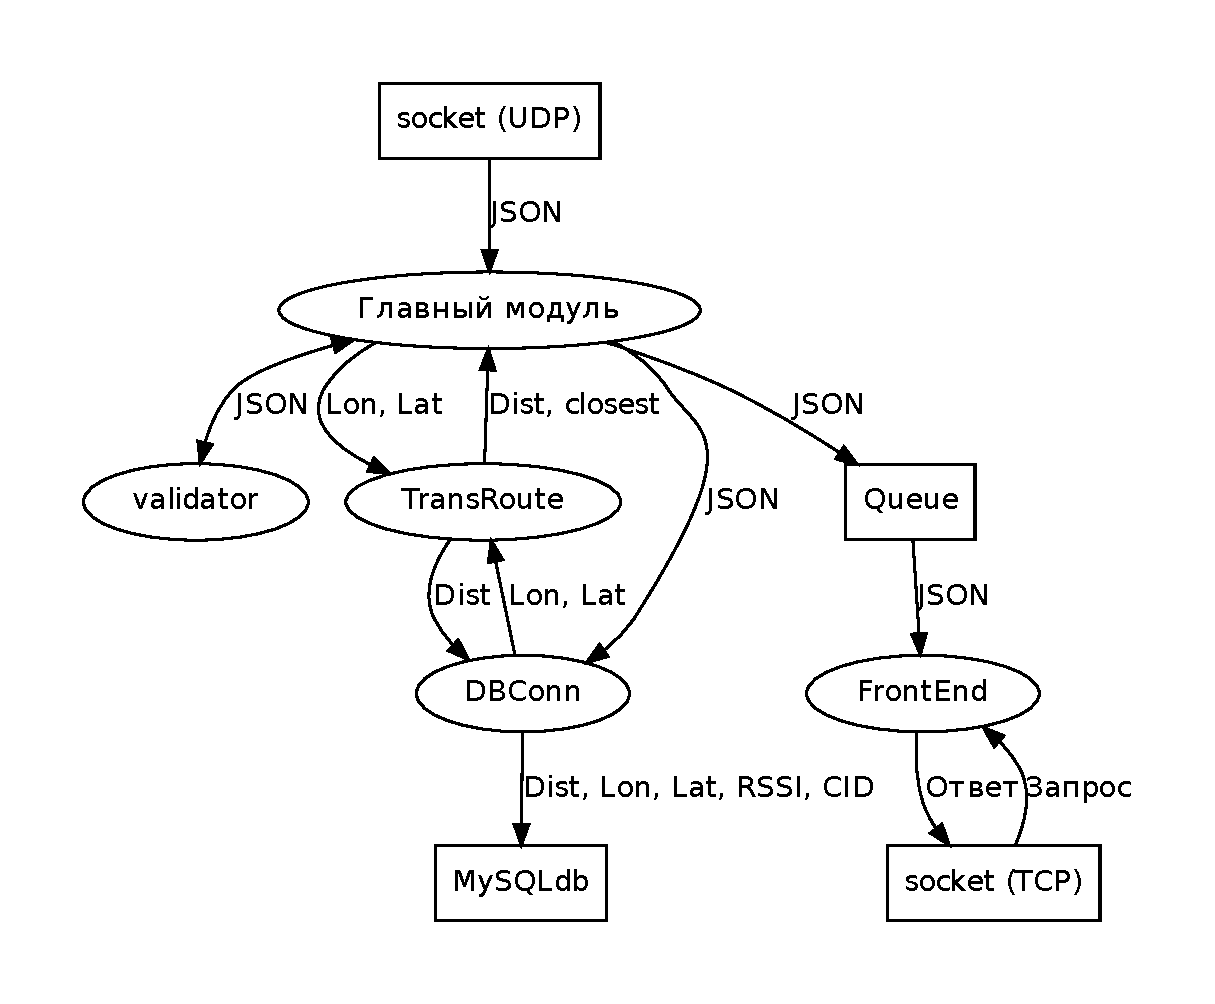
\includegraphics[height=0.8\textheight]{server-collect-dataflow.pdf}}
}

\frame{
	\frametitle{Режим позиционирования}
	\centerline{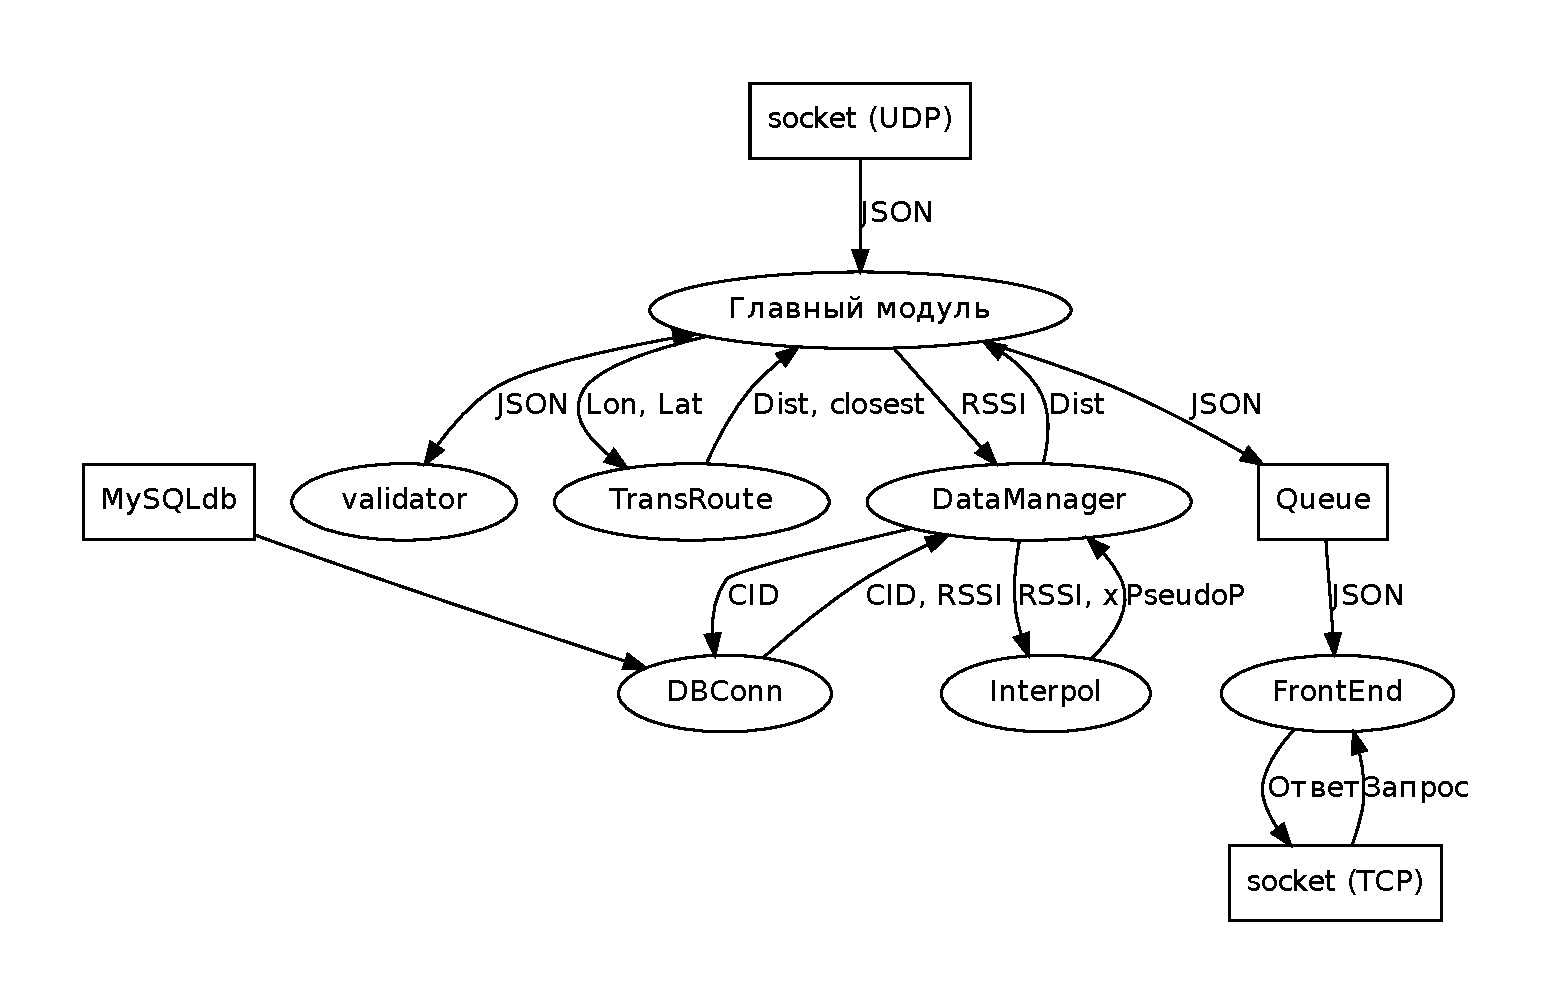
\includegraphics[height=0.8\textheight]{server-perform-dataflow.pdf}}
}

\frame{
	\frametitle{Мобильное приложение}
	\centerline{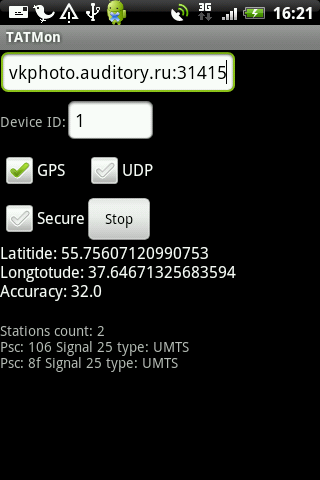
\includegraphics[height=0.8\textheight]{TATMon-android.png}}
}


\begin{frame}[fragile]
	\frametitle{Пример сообщения}
	\begin{lstlisting}
{	"GSM":{
		"cellcount":2, 
		"cells":[
				{"CID":11531, "Psc":-1, "RSSI":26, "type":"EDGE"}, 
				{"CID":32779, "Psc":-1, "RSSI":22, "type":"EDGE"}
			]
		},
	"GPS": {
			"lng":37.64814019203186,
			"ltd":55.75437605381012,
			"acc":24.0
		}}
	\end{lstlisting}
\end{frame}

\frame{
	\frametitle{Вход алгоритма}
	\begin{equation}
		data = \begin{pmatrix}
			Dist_0 & RSSI_0 \\
			Dist_1 & RSSI_1 \\
			\vdots & \vdots \\
    Dist_{len(data)-1} & RSSI_{len(data)-1}
		\end{pmatrix}
		\nonumber
		\label{eq:data-create-vars}
	\end{equation}
}

\frame{
	\frametitle{Создание переменных}
		\begin{equation}
			self.X = \begin{pmatrix}
				1 & Dist_0 & Dist_0^2 & \cdots & Dist_0^{order} \\
				1 & Dist_1 & Dist_1^2 & \cdots & Dist_1^{order} \\
      \vdots & \vdots & \vdots & \vdots & \vdots \\
				       1 & Dist_{len(data)-1} & Dist_{len(data)-1}^2 & \cdots & Dist_{len(data)-1}^{order}
			\end{pmatrix}
			\label{eq:self-x-create-vars}
			\nonumber
		\end{equation}

		\begin{equation}
			self.Y = \begin{pmatrix}
				RSSI_0 \\
				RSSI_1 \\
				\vdots \\
				RSSI_{len(data)-1}
			\end{pmatrix}
			\nonumber
			\label{eq:self-y-create-vars}
		\end{equation}
}

\begin{frame}[fragile]
	\frametitle{Нормальные уравнения}
	\begin{equation}
		self.theta = (self.X^\intercal \cdot self.X)^{+} \cdot self.X^\intercal \cdot self.Y
		\nonumber
		\label{eq:solve-theta}
	\end{equation}
\begin{lstlisting}
def solve_theta(self):
    self.theta = numpy.transpose(self.X)
    self.theta = numpy.dot(self.theta, self.X)
    self.theta = numpy.linalg.pinv(self.theta)
    self.theta = numpy.dot(self.theta,\
        numpy.transpose(self.X))
    self.theta = numpy.dot(self.theta, self.Y)
\end{lstlisting}
\end{frame}
\setcounter{framenumber}{\value{finalframe}}

\end{document}


